\subsection{Analisis Benchmark}
\label{subsection:analisis-benchmark}

Analisis \textit{benchmark} dilakukan untuk mengevaluasi kinerja sistem yang telah diimplementasikan. Analisis dilakukan dengan menggunakan data hasil \textit{benchmark} yang telah dibuat dengan sistem pada Bagian \ref{subsubsection:implementasi-benchmark}. Analisis akan dimulai dari analisis operasi \textit{write}, dilanjut dengan analisis operasi \textit{read}, dan diakhiri dengan analisis keseluruhan dari sistem.

\subsubsection{Setup Benchmark}
\label{subsubsection:setup-benchmark}

Pengaturan variabel yang digunakan dalam \textit{benchmark} dilakukan pada file \textit{scripts.js} seperti yang sudah dijelaskan pada bagian \ref{subsubsection:implementasi-benchmark}. Skenario \textit{benchmark} dibagi menjadi tiga dengan mempertimbangkan hipotesis pengaruh variabel yang dinyatakan pada bagian \ref{sec:rumusan-masalah}. Skenario tersebut adalah sebagai berikut:

\begin{enumerate}
  \item Internet cepat dan \textit{payload} kecil
  
  Skenario ini menggambarkan kondisi ekstrim berlawanan dengan hipotesis yang berpihak pada kinerja replikasi. Skenario ini digunakan untuk menguji apakah sistem \textit{erasure coding} masih dapat bersaing dengan sistem replikasi serta melihat keuntungan dari penggunaan replikasi dalam kondisi tersebut. 

  \item Internet rata-rata dan \textit{payload} umum
  
  Skenario ini bertujuan untuk mencari kondisi perbatasan antara kinerja \textit{erasure coding} dan replikasi. Tujuannya adalah untuk mencari poin ketika sistem \textit{erasure coding} mulai mengungguli sistem replikasi ataupun sebaliknya. Skenario ini juga diharapkan dapat memberikan gambaran umum pengaruh variabel-variabel yang ada terhadap kinerja sistem.
  
  \item Internet lambat dan \textit{payload} umum
  
  Skenario ini menggambarkan kondisi ekstrim berlawanan dengan hipotesis yang berpihak pada kinerja \textit{erasure coding}. Skenario ini digunakan untuk menguji apakah sistem replikasi masih dapat bersaing dengan sistem \textit{erasure coding} serta melihat keuntungan dari penggunaan \textit{erasure coding} dalam kondisi tersebut .

\end{enumerate}

Dari skenario-skenario tersebut, diturunkan beberapa variabel yang akan digunakan pada \textit{benchmark}. Menggunakan sistem \textit{benchmark} yang telah dibuat, variabel ini akan dijalankan untuk semua kombinasi yang dapat dibentuk. Variabel-variabel tersebut dapat dilihat pada tabel \ref{tab:variabel-benchmark}.

\begin{table}[ht]
  \centering
  \caption{Variabel yang digunakan pada \textit{benchmark}}
  \label{tab:variabel-benchmark}
  \begin{tabular}{|c|p{6cm}|p{6cm}|}
    \hline
    \textbf{Skenario} & \textbf{Ukuran \textit{Payload}} & \textbf{Bandwidth} \\ \hline
    1 & 1024 B & 10 Gbps \\ \hline
    2 & 200 KB, 400 KB, 600 KB, 800 KB, 1 MB & 10 Mbps, 25 Mbps, 40 Mbps, 55 Mbps, 70 Mbps \\ \hline
    3 & 200 KB, 400 KB, 600 KB, 800 KB, 1 MB & 256 kbps \\ \hline
  \end{tabular}
\end{table}

Terkait ukuran \textit{payload}, nilai yang diambil adalah berdasarkan ukuran \textit{payload} yang umum digunakan pada aplikasi \textit{key-value store} seperti yang dijelaskan pada bagian \ref{sec:key-value-database}. Penambahan linear dilakukan untuk mempermudah analisis data dan mendapatkan pola yang lebih jelas. Selain itu, untuk bandwidth, nilai yang diambil adalah berdasarkan kecepatan internet yang umum digunakan di Indonesia lalu dilakukan penambahan linear dengan alasan yang sama. Nilai-nilai tersebut diambil dari data yang tersedia pada situs Speedtest Global Index\footnote{\url{https://www.speedtest.net/global-index}}.
\subsubsection{Analisis Operasi Write}
\label{subsubsection:analisis-operasi-write}

Analisis kinerja operasi \textit{write} merupakan inti dari penilitian ini, seperti yang sudah dijelaskan pada bagian \ref{sec:rumusan-masalah}. Analisis ini bertujuan untuk memvalidasi bahwa \textit{erasure coding} dapat mengungguli replikasi dalam kondisi tertentu. Analisis kinerja operasi \textit{write} akan dibagi berdasarkan skenario yang sudah disebutkan pada bagian \ref{subsubsection:setup-benchmark}. Setiap skenario akan dianalisis berdasarkan hasil \textit{benchmark} yang telah dilakukan.

\begin{enumerate}
  \item Skenario 1: Internet cepat dan \textit{payload} kecil

  Pada skenario pertama yang dirancang sebagai kondisi ekstrem yang menguntungkan replikasi, hasil \textit{benchmark} menunjukkan bahwa sistem replikasi memiliki \textit{response time} yang lebih rendah dibandingkan sistem berbasis \textit{erasure coding}. Perbedaan kinerja ini dapat dilihat pada gambar \ref{fig:write-smload-fastnet}.

  \begin{figure}[ht]
      \centering
      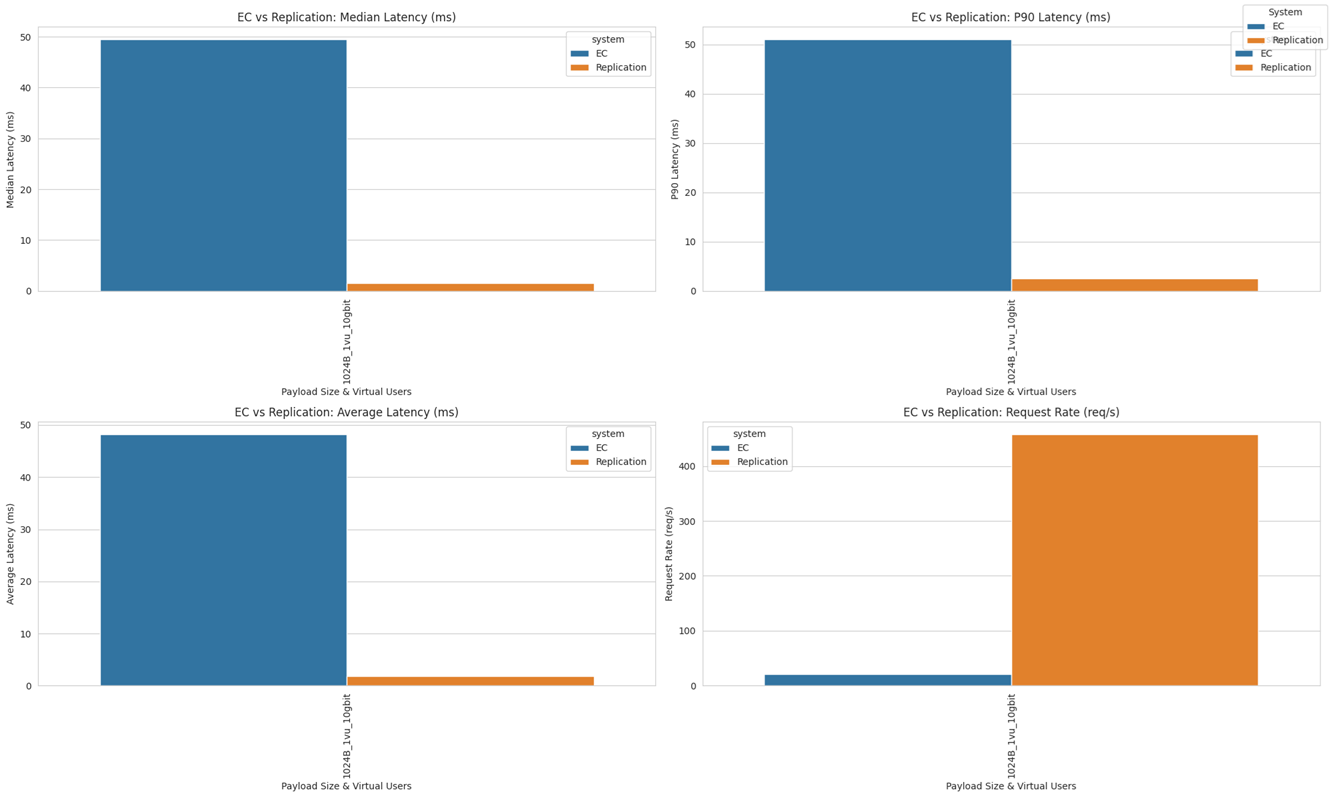
\includegraphics[width=0.8\textwidth]{resources/chapter-4/write_smload_fastnet.png}

      \caption{Kinerja Operasi Write pada Internet Cepat dan Payload Kecil}
      \label{fig:write-smload-fastnet}
  \end{figure}
  
  Interpretasi dari hasil ini terletak pada dinamika komponen latensi. Pada jaringan dengan \textit{bandwidth} tinggi seperti 10 Gbps, waktu yang dibutuhan untuk mentransfer data menjadi kecil. Selain itu, data yang kecil membuat operasi terkait data seperti penulisan pada \textit{memory} dan \textit{disk} menjadi kecil juga. Dengan kecilnya waktu transfer dan operasi terkait data, faktor penentu \textit{response time} adalah biaya komputasi dan \textit{overhead} pemrosesan pada setiap node.

  Dalam skenario ini, proses \textit{erasure coding} yang lebih kompleks membutuhkan waktu yang lebih lama dibandingkan dengan proses replikasi yang lebih sederhana. Lingkungan seperti ini umum ditemukan pada komunikasi antar-\textit{server} dalam satu pusat data modern dengan penggunaan transaksi data berukuran kecil seperti pembaruan metadata, status sesi, atau operasi konfigurasi singkat.
  
  \item Skenario 2: Internet lambat dan \textit{payload} besar
  
  Skenario kedua dirancang sebagai kondisi ekstrem yang berlawanan dengan skenario pertama dengan keuntungan pada \textit{erasure coding}. Hasil \textit{benchmark} pada skenario ini menunjukkan pembalikan kinerja dramatis dengan sistem berbasis \textit{erasure coding} secara konsisten mengungguli replikasi dengan \textit{response time} yang lebih rendah untuk \textit{payload} yang diuji. Gambar \ref{fig:write-bigload-slownet} menunjukkan perbandingan kinerja operasi \textit{write} pada skenario ini.

  \begin{figure}[ht]
      \centering
      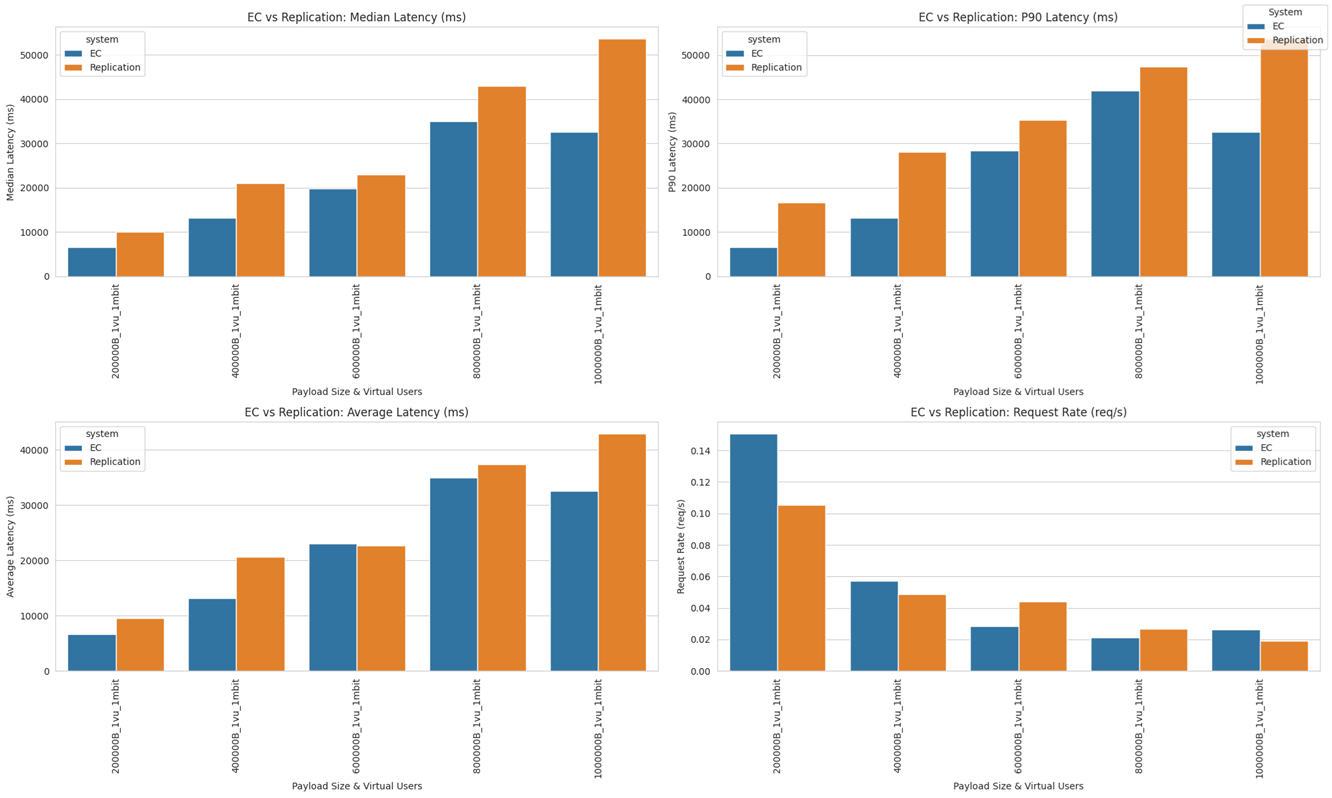
\includegraphics[width=0.8\textwidth]{resources/chapter-4/write_bigload_slownet.png}

      \caption{Kinerja Write pada Internet Lambat dan Payload Besar}
      \label{fig:write-bigload-slownet}
  \end{figure}

  Hasil dari skenario ini mengkonfirmasi bahwa \textit{erasure coding} dapat mengungguli replikasi dalam kondisi tertentu, yaitu dalam skenario dengan \textit{bandwidth} rendah dan untuk \textit{payload} yang besar. Dalam kondisi ini, waktu transfer data menjadi faktor dominan dalam \textit{response time}. Proses \textit{erasure coding} walaupun lebih kompleks, dapat memberikan \textit{latensi} lebih cepat karena mengurangi jumlah data yang harus ditransfer serta dioperasikan. Lingkungan seperti ini umum ditemukan pada aplikasi yang beroperasi dengan sumber daya jaringan terbatas, seperti aplikasi \textit{internet of things} yang tersebar di area luas, \textit{edge computing}, atau pencadangan data melalui koneksi internet yang lambat. 

  \item Skenario 3: Internet menengah dan \textit{payload} besar
  
  Dengan didapatkannya bahwa \textit{erasure coding} dapat mengungguli replikasi pada skenario kedua, skenario ketiga dirancang untuk mengeksplorasi titik perbatasan ketika keunggulan kinerja beralih dari sistem \textit{erasure coding} ke sistem replikasi. Seperti yang sudah dijelaskan pada bagian \ref{subsubsection:setup-benchmark}, skenario ini dirancang dengan merepresentasikan kondisi jaringan dengan \textit{bandwidth} rata-rata internet di Indonesia pada saat penulisan, yaitu 40 Mbps, dengan penambahan atau pengurangan linear.
  
  \begin{figure}[ht]
    \centering
    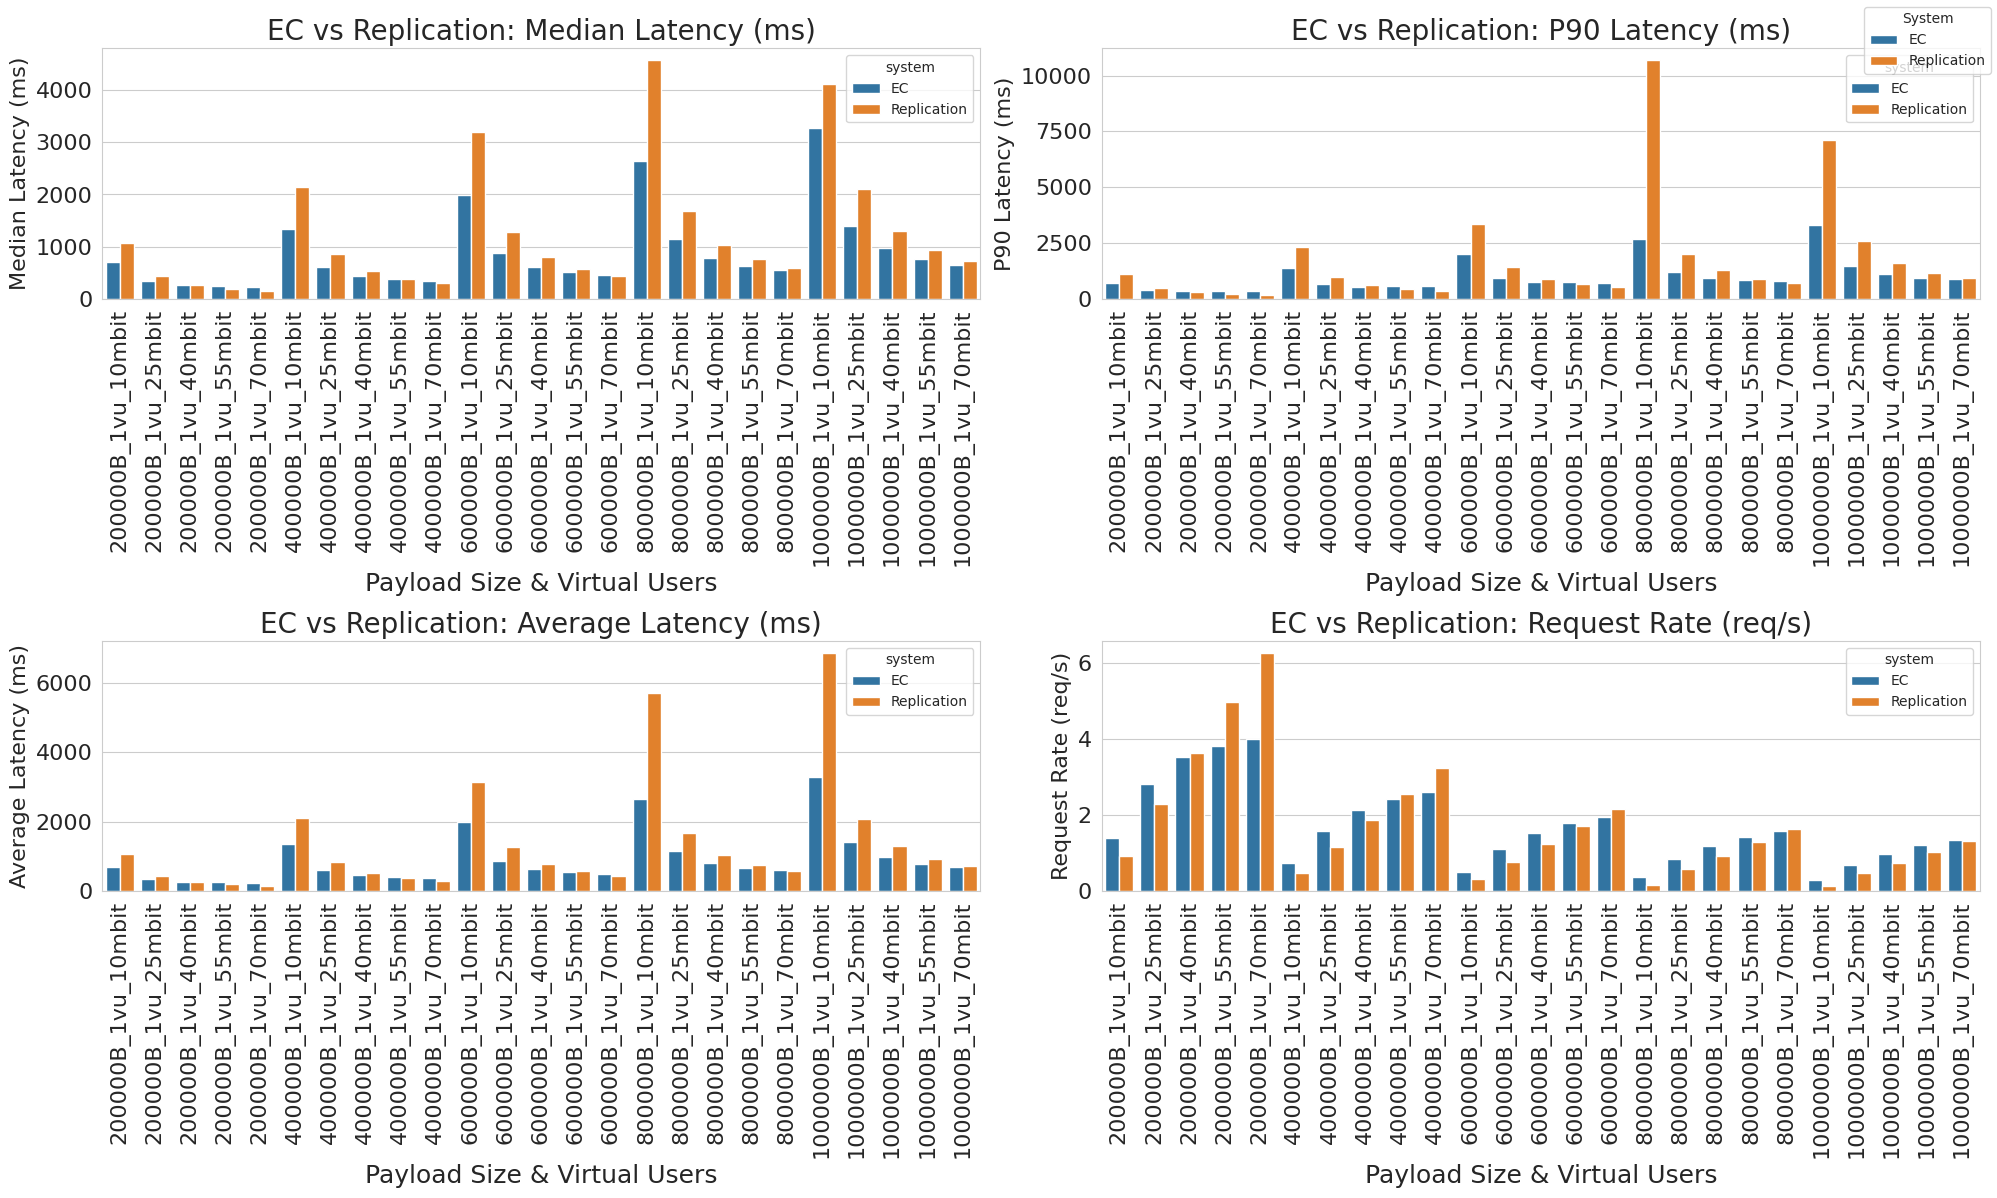
\includegraphics[width=0.8\textwidth]{resources/chapter-4/write_bigload_avgnet.png}

    \caption{Kinerja Write pada Internet Menengah dan Payload Besar}
    \label{fig:write-bigload-avgnet}
  \end{figure}

  Skenario ini menggunakan kombinasi \textit{payload} dan \textit{bandwidth} yang beragam sehingga memberikan diagram dengan grafik yang lebih kompleks. Gambar \ref{fig:write-bigload-avgnet} menunjukkan hasil \textit{benchmark} untuk skenario ini. Dari grafik tersebut, terlihat bahwa keunggulan \textit{erasure coding} semakin berkurang seiring dengan peningkatan \textit{bandwidth} dan penurunan ukuran \textit{payload}. Pada titik tertentu, sistem berbasis replikasi mulai mengungguli sistem berbasis \textit{erasure coding}. Titik impas terjadi ketika penghematan waktu dari transfer data yang lebih sedikit pada \textit{erasure coding} setara dengan penambahan waktu dari proses komputasi \textit{encoding}.

  \begin{figure}[ht]
    \centering
    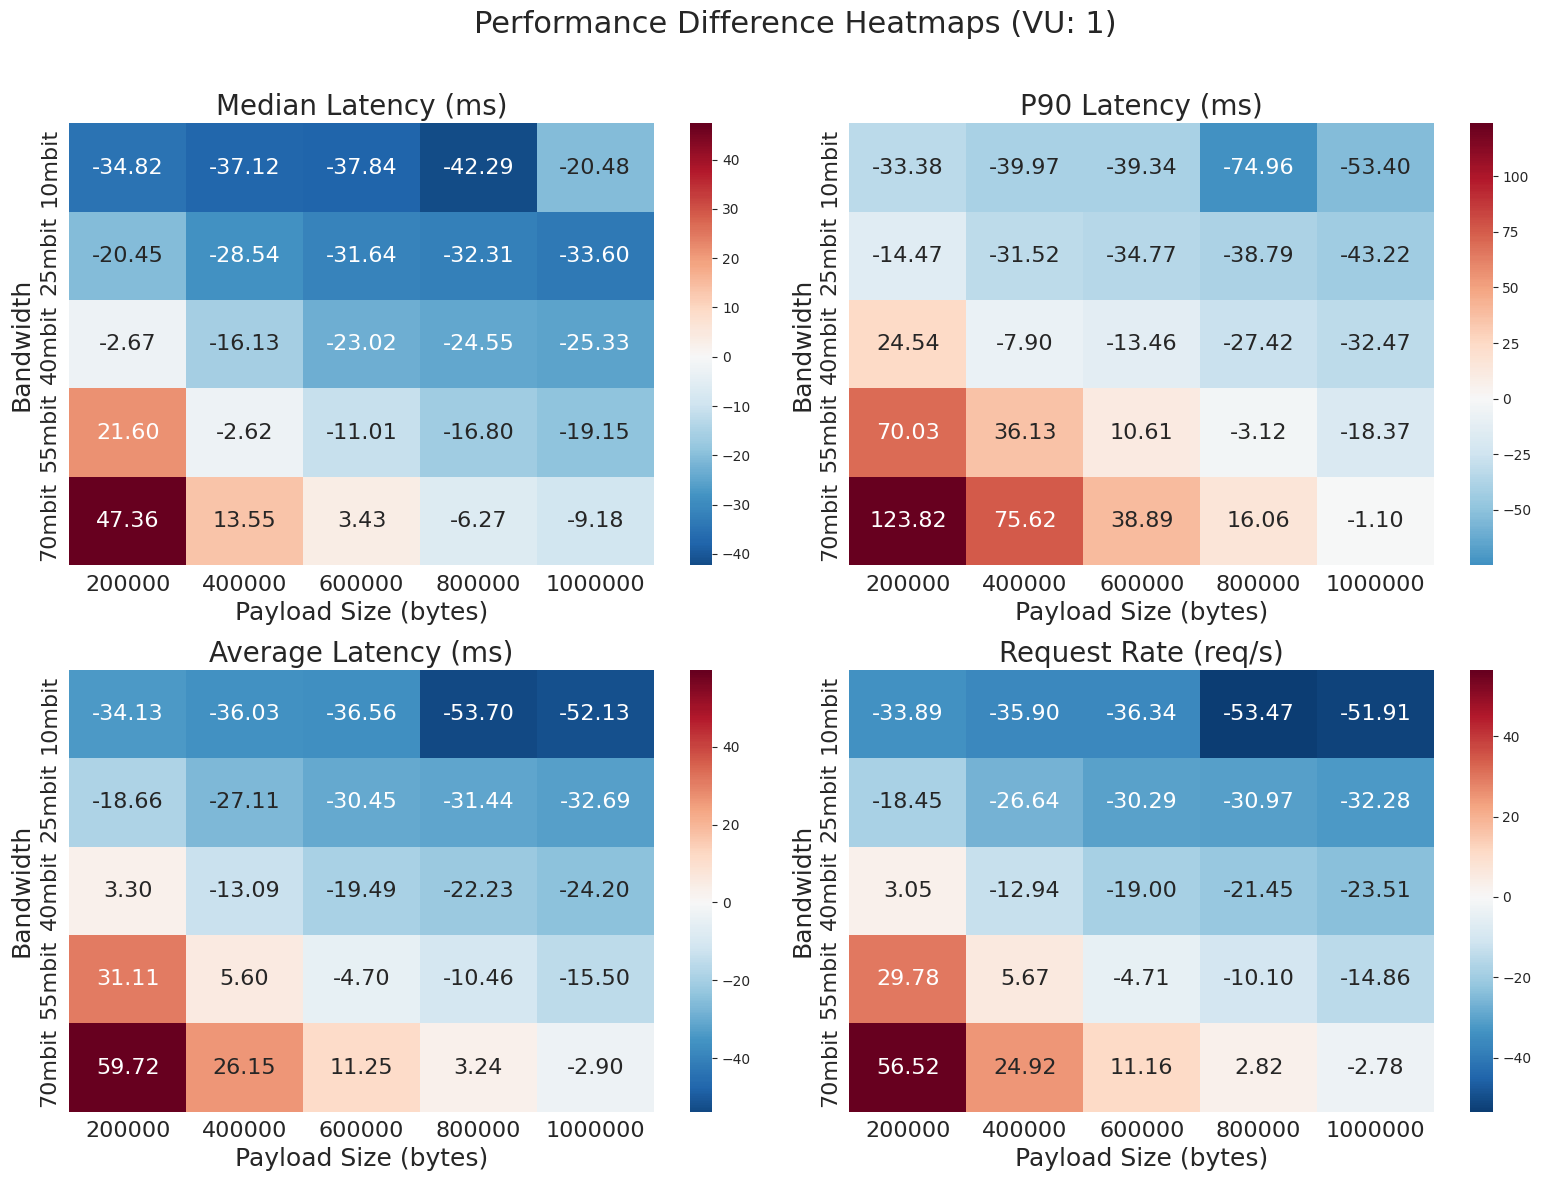
\includegraphics[width=0.8\textwidth]{resources/chapter-4/write_bigload_avgnet_heatmap.png}

    \caption{Heatmap Write pada Internet Menengah dan Payload Besar}
    \label{fig:write-bigload-avgnet-heatmap}
  \end{figure}

  Untuk memudahkan visualisasi, gambar \ref{fig:write-bigload-avgnet-heatmap} menunjukkan rasio kinerja dari hasil \textit{benchmark} terhadap \textit{payload} dan \textit{bandwidth} yang digunakan dalam persen. Warna biru dan nilai negatif menunjukkan keunggulan sistem berbasis \textit{erasure coding}, sedangkan warna merah dan nilai positif menunjukkan keunggulan sistem berbasis replikasi. Titik impas terlihat pada area transisi antara warna biru dan merah.  Kode yang digunakan untuk menghasilkan gambar ini dapat dilihat pada lampiran \ref{appendix:write-benchmark-code}. Transisi ini dapat dilihat pada gambar tersebut, namun tidak didapat titik yang tepat.

  Untuk menggambarkan perolehan titik impas, dapat dibuat diagram garis yang menunjukkan rata-rata \textit{response time} sistem berbasis \textit{erasure coding} dan replikasi terhadap \textit{bandwidth} dan ukuran \textit{payload}. Gambar \ref{fig:write-bigload-avgnet-line} menunjukkan diagram garis tersebut. Diagram ini memberikan gambaran visual yang jelas tentang bagaimana kinerja kedua sistem berubah seiring dengan variasi \textit{bandwidth} dan ukuran \textit{payload}.

  \begin{figure}[ht]
    \centering
    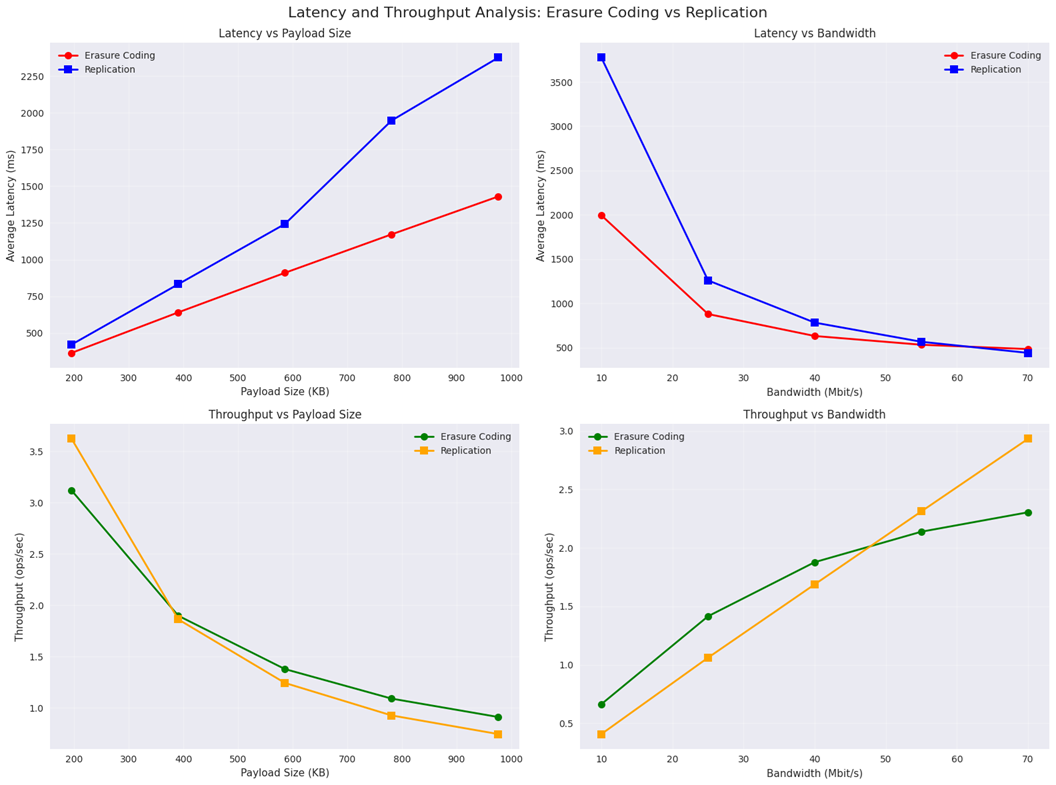
\includegraphics[width=0.8\textwidth]{resources/chapter-4/write_bigload_avgnet_line.png}

    \caption{Diagram Garis Write pada Internet Menengah dan Payload Besar}
    \label{fig:write-bigload-avgnet-line}
  \end{figure}

  
  Namun, untuk mendapatkan nilai yang tepat untuk titik impas antara sistem berbasis \textit{erasure coding} dan sistem berbasis replikasi, perlu dilakukan analisis lebih lanjut. Analisis untuk mendapatkan titik impas dilakukan secara menurunkan hasil \textit{benchmark} yang sudah dilakukan menjadi fungsi menggunakan pendekatan regresi. Fungsi ini kemudian digunakan untuk memperkirakan titik impas. Sebelum melakukan regresi, perlu dilihat \textit{scatter plot} dari hasil \textit{benchmark} sebagai gambaran visual relasi antara \textit{bandwidth}, ukuran \textit{payload}, dan \textit{response time}. Gambar \ref{fig:write-bigload-avgnet-scatter} menunjukkan \textit{scatter plot} tersebut.

  \begin{figure}[ht]
    \centering
    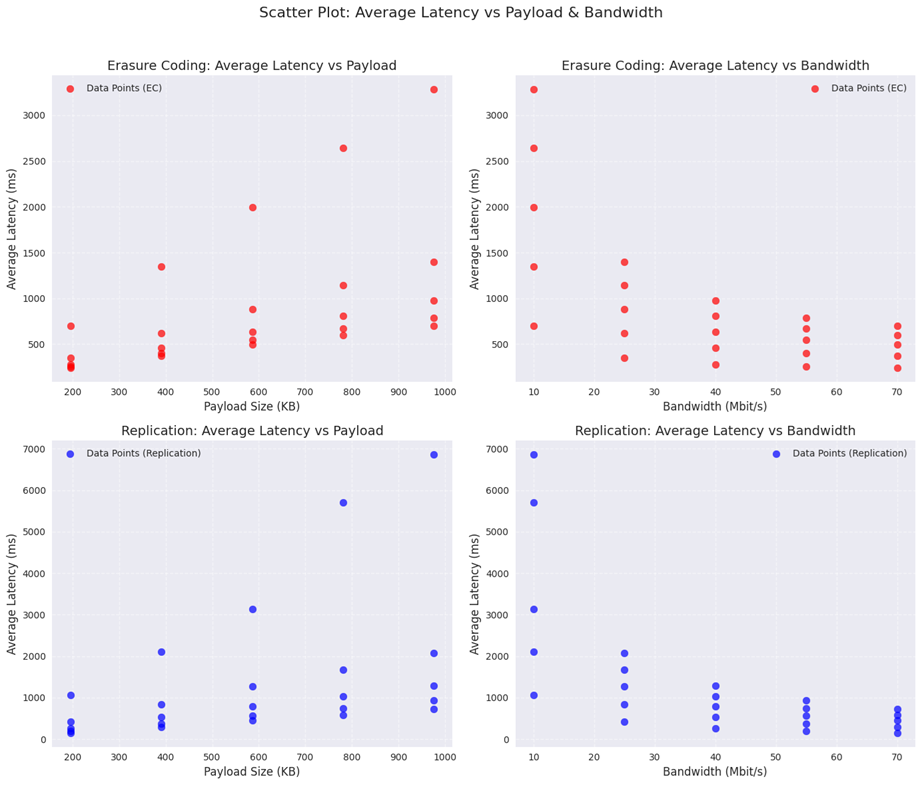
\includegraphics[width=0.8\textwidth]{resources/chapter-4/write_bigload_avgnet_scatterplot.png}

    \caption{Scatter Plot Write pada Internet Menengah dan Payload Besar}
    \label{fig:write-bigload-avgnet-scatter}
  \end{figure}

  Dari \textit{scatter plot} tersebut, terlihat bahwa hubungan dari \textit{bandwidth} dan ukuran \textit{payload} terhadap \textit{response time} tidak linear. Data yang dimiliki hanya sedikit, yaitu 25 data, sehingga regresi yang dilakukan harus mempertimbangkan risiko \textit{overfitting} yang tinggi. Selain itu, disebabkan lingkungan eksperimen dilakukan pada komputer pribadi, \textit{noise} dari eksperimen dapat mempengaruhi hasil. Dengan mempertimbangkan semua hal tersebut, regresi dilakukan dengan model \textit{ridge regression}. Model ini dipilih karena dapat menangani data yang memiliki banyak \textit{noise} serta mengurangi risiko \textit{overfitting} dengan menambahkan bias pada model regresi.

  Model \textit{ridge regression} gabungan dari \textit{bandwidth} dan \textit{payload} terhadap \textit{response time} menghasilkan model tiga dimensi seperti yang ditunjukkan pada gambar \ref{fig:write-bigload-avgnet-regression}.

  \begin{figure}[ht]
    \centering
    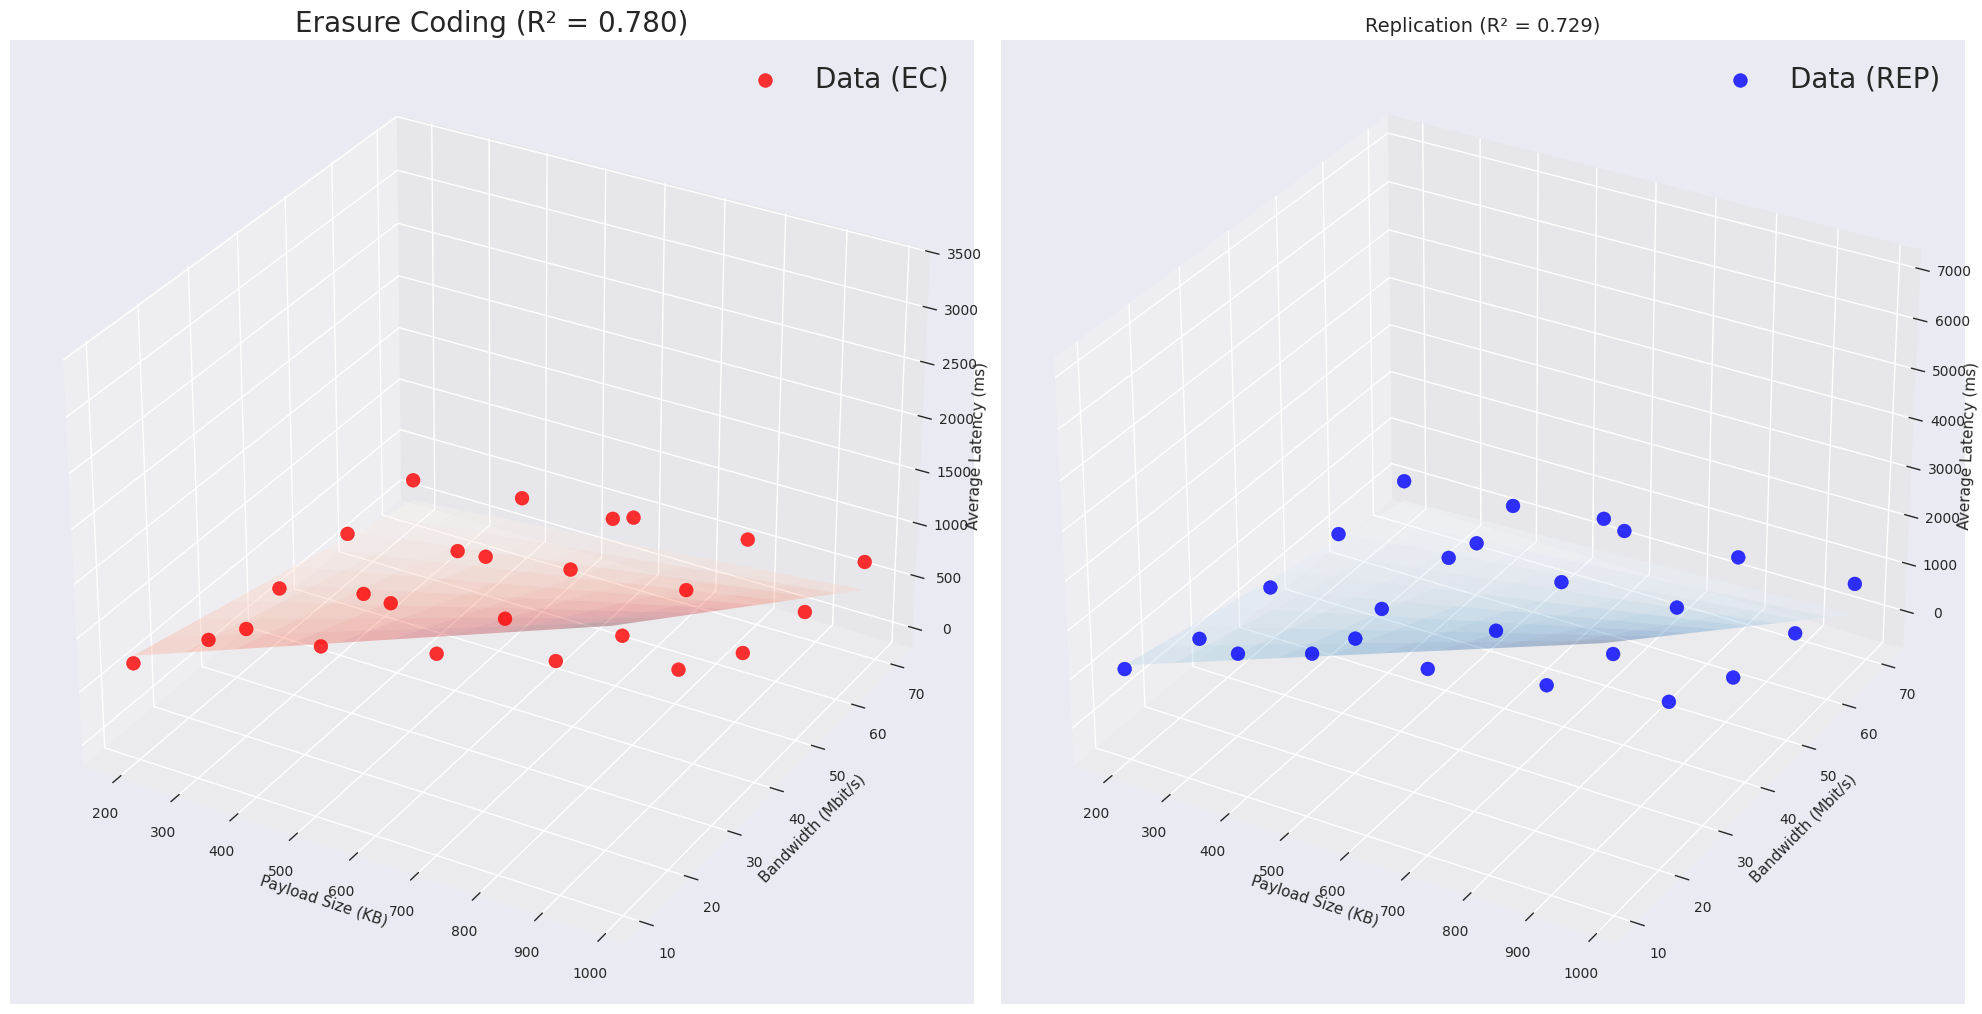
\includegraphics[width=0.8\textwidth]{resources/chapter-4/write_bigload_avgnet_regression.png}

    \caption{Model Regresi Operasi Write}
    \label{fig:write-bigload-avgnet-regression}
  \end{figure}

  Dari model regresi yang dilakukan, kurva pendekatan titik impas antara sistem berbasis \textit{erasure coding} dan sistem berbasis replikasi dapat dihasilkan dengan mencari perpotongan dari model regresi tersebut. Perpotongan didapat dengan menggunakan selisih dan selisih bernilai nol merupakan titik impas. Gambar \ref{fig:write-bigload-avgnet-boundary} menunjukkan analisis titik impas yang dilakukan dengan menggunakan model regresi. Dari perpotongan tersebut dapat dimodelkan menjadi persamaan kurva matematis yang dapat digunakan untuk memperkirakan titik impas pada \textit{bandwidth} dan ukuran \textit{payload} tertentu dengan nilai di atas kurva berarti sistem berbasis \textit{erasure coding} mengungguli sistem berbasis replikasi, dan nilai di bawah kurva berarti sebaliknya.


  \begin{figure}[ht]
    \centering
    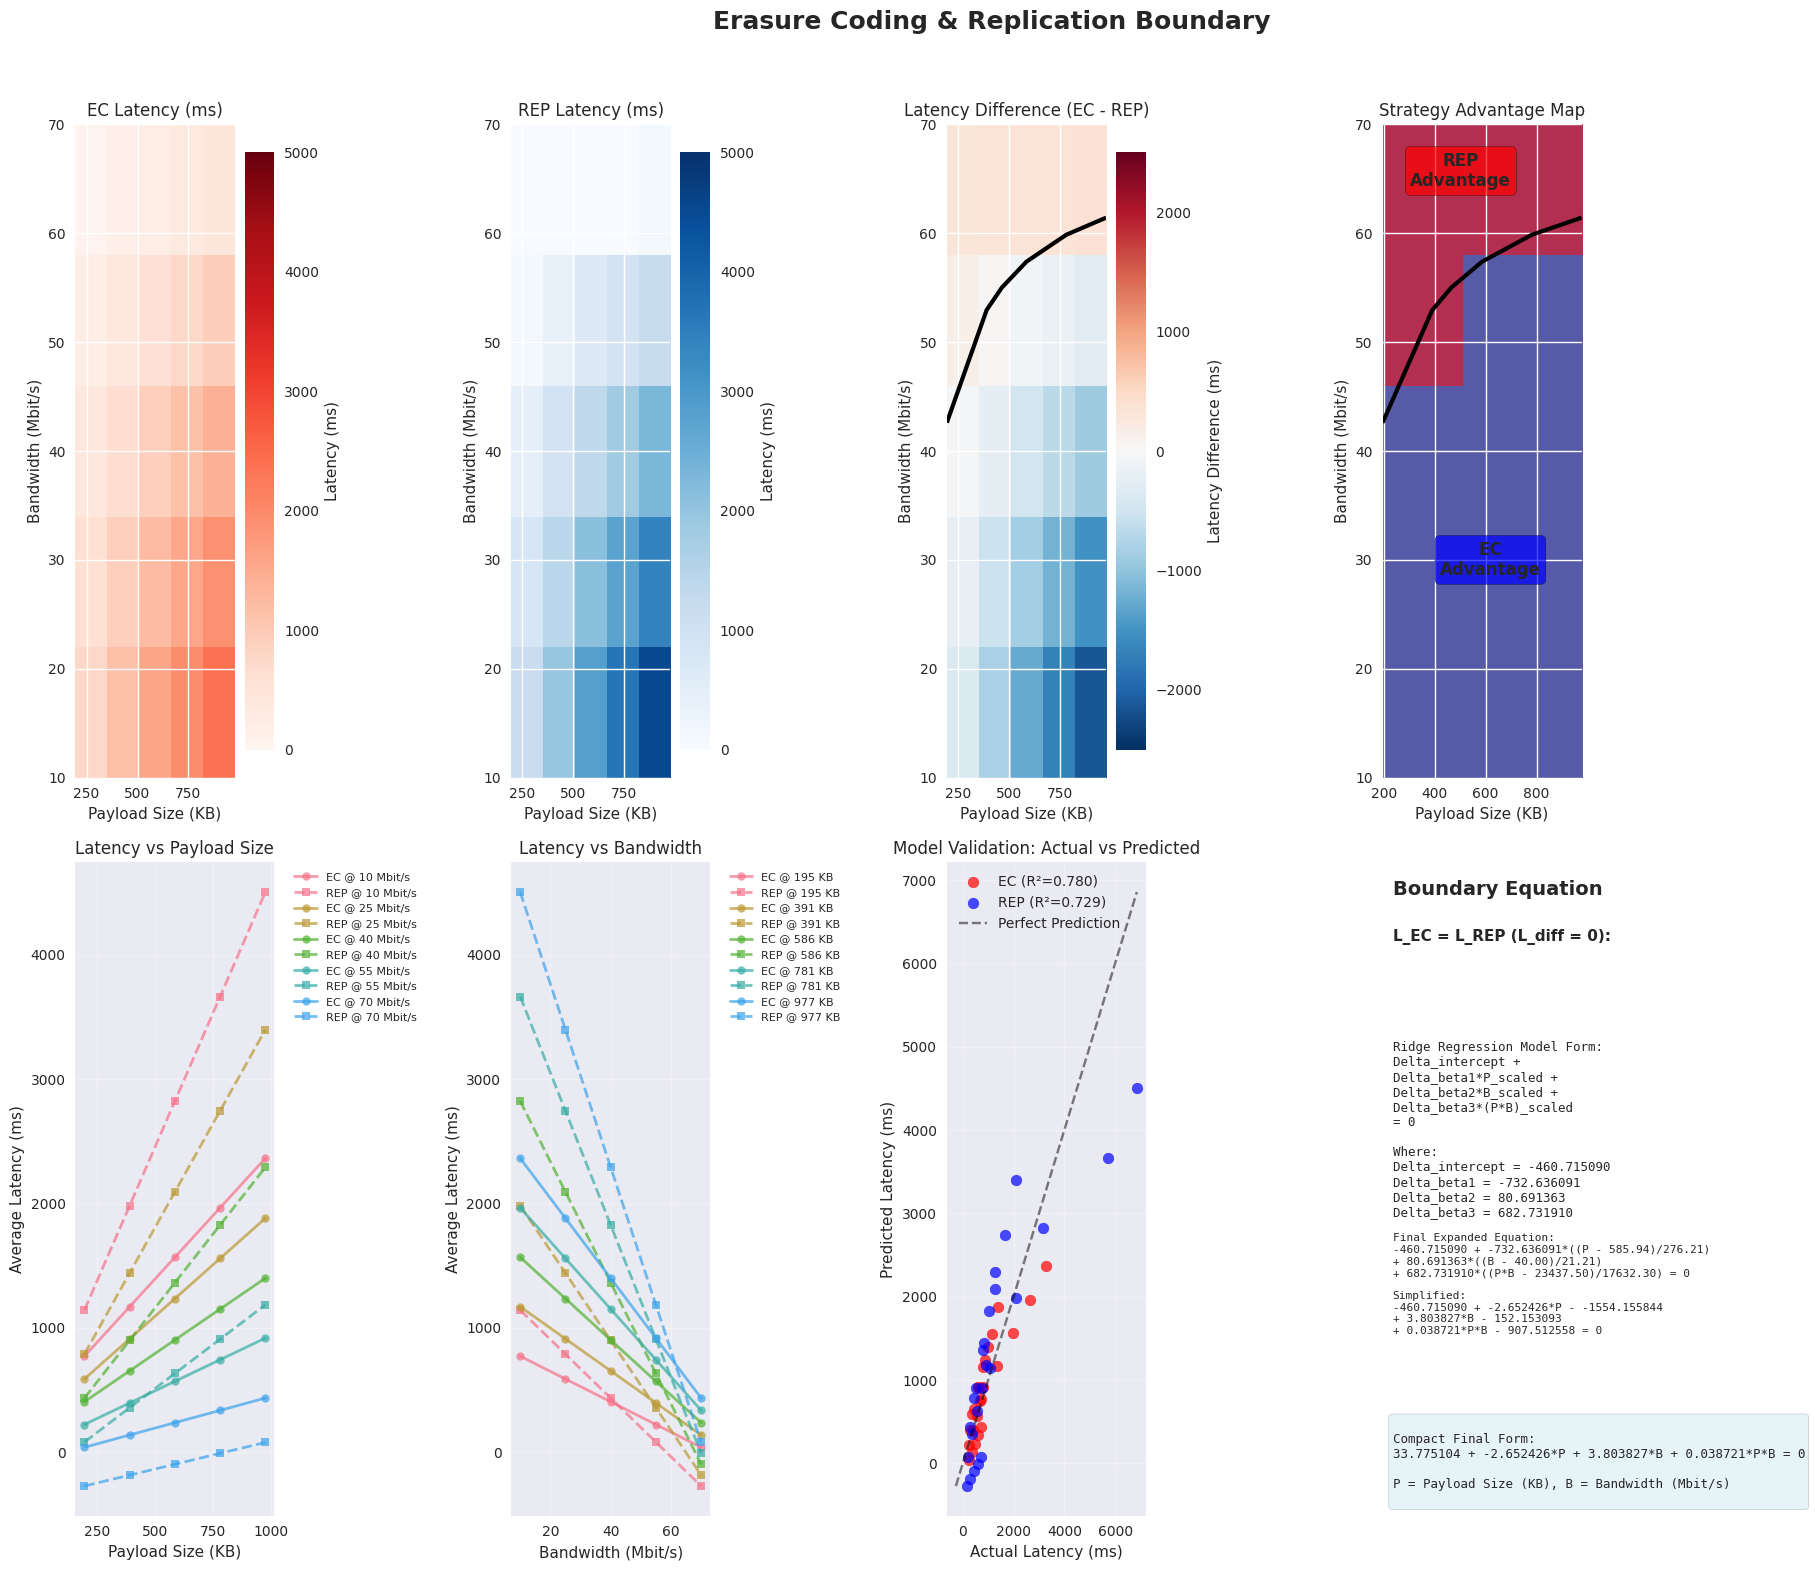
\includegraphics[width=\textwidth]{resources/chapter-4/write_bigload_avgnet_boundary.png}

    \caption{Analisis Titik Impas pada Operasi Write}
    \label{fig:write-bigload-avgnet-boundary}
  \end{figure}

  Kode yang digunakan untuk melakukan regresi ini dapat dilihat pada lampiran \ref{appendix:write-regression-code}. Perlu diketahui juga bahwa model regresi ini tidak mempertimbangkan faktor lain seperti kecepatan komputasi dari sistem yang digunakan, kecepatan akses memori, kecepatan akses disk, ataupun faktor lain yang dapat mempengaruhi \textit{response time}. Model ini hanya valid pada kondisi dan lingkungan eksperimen yang dilakukan.

\end{enumerate}

\subsubsection{Analisis Operasi Read}
\label{subsubsection:analisis-operasi-read}

Berbeda secara hipotesis dengan operasi \textit{write}, hipotesis kinerja operasi \textit{read} adalah bahwa replikasi akan secara konsisten menunjukkan kinerja yang lebih unggul dalam kondisi normal. Hal ini disebabkan oleh kompleksitas \textit{erasure coding} yang membutuhkan rekonstruksi data dari beberapa bagian, sedangkan replikasi dapat mengembalikan data secara langsung dari salinan pada \textit{node} tersebut.

Pada implementasi yang dijelaskan pada Bagian \ref{subsubsection:implementasi-memory-store}, dibuat sebuah \textit{in-memory store} untuk mengurangi latensi \textit{read} dengan mengurangi operasi rekonstruksi data. Jika menggunakan hal tersebut, \textit{erasure coding} akan memiliki kinerja yang setara dengan replikasi ketika data yang dibutuhkan sudah ada di \textit{in-memory store}. Untuk keperluan analisis ini, \textit{in-memory store} diabaikan dan semua \textit{request} yang diterima perlu direkonstruksi terlebih dahulu pada sistem \textit{erasure coding}.

Analisis ini bertujuan untuk mengukur seberapa buruk kinerja operasi \textit{read} pada sistem \textit{erasure coding} dibandingkan dengan replikasi. Sama seperti analisis operasi \textit{write}, analisis ini akan dibagi berdasarkan skenario yang sudah disebutkan pada Bagian \ref{subsubsection:setup-benchmark}. Setiap skenario akan dianalisis berdasarkan hasil \textit{benchmark} yang telah dilakukan.

\begin{enumerate}
  \item Skenario 1: Internet cepat dan \textit{payload} kecil
  
  Pada skenario pertama yang dirancang sebagai kondisi ekstrem yang menguntungkan replikasi, hasil \textit{benchmark} menunjukkan bahwa sistem replikasi memiliki \textit{response time} yang lebih rendah dibandingkan sistem berbasis \textit{erasure coding}. Skenario ini mengkonfirmasi hipotesis bahwa replikasi akan lebih cepat dalam kondisi internet cepat dan \textit{payload} kecil untuk operasi \textit{read}.
  
  Tidak banyak yang dapat disimpulkan dari hasil ini, karena skenario ini dirancang untuk menguntungkan replikasi dan dengan hipotesis menyebutkan bahwa replikasi akan selalu lebih cepat dalam kondisi apapun dibandingkan dengan \textit{erasure coding} untuk operasi \textit{read}. Skenario ini adalah salah satu dari kemungkinan kondisi untuk menjalankan sistem berbasis \textit{erasure coding} ataupun replikasi. Perbedaan kinerja ini dapat dilihat pada Gambar \ref{fig:read-smload-fastnet}.

  \begin{figure}[ht]
    \centering
    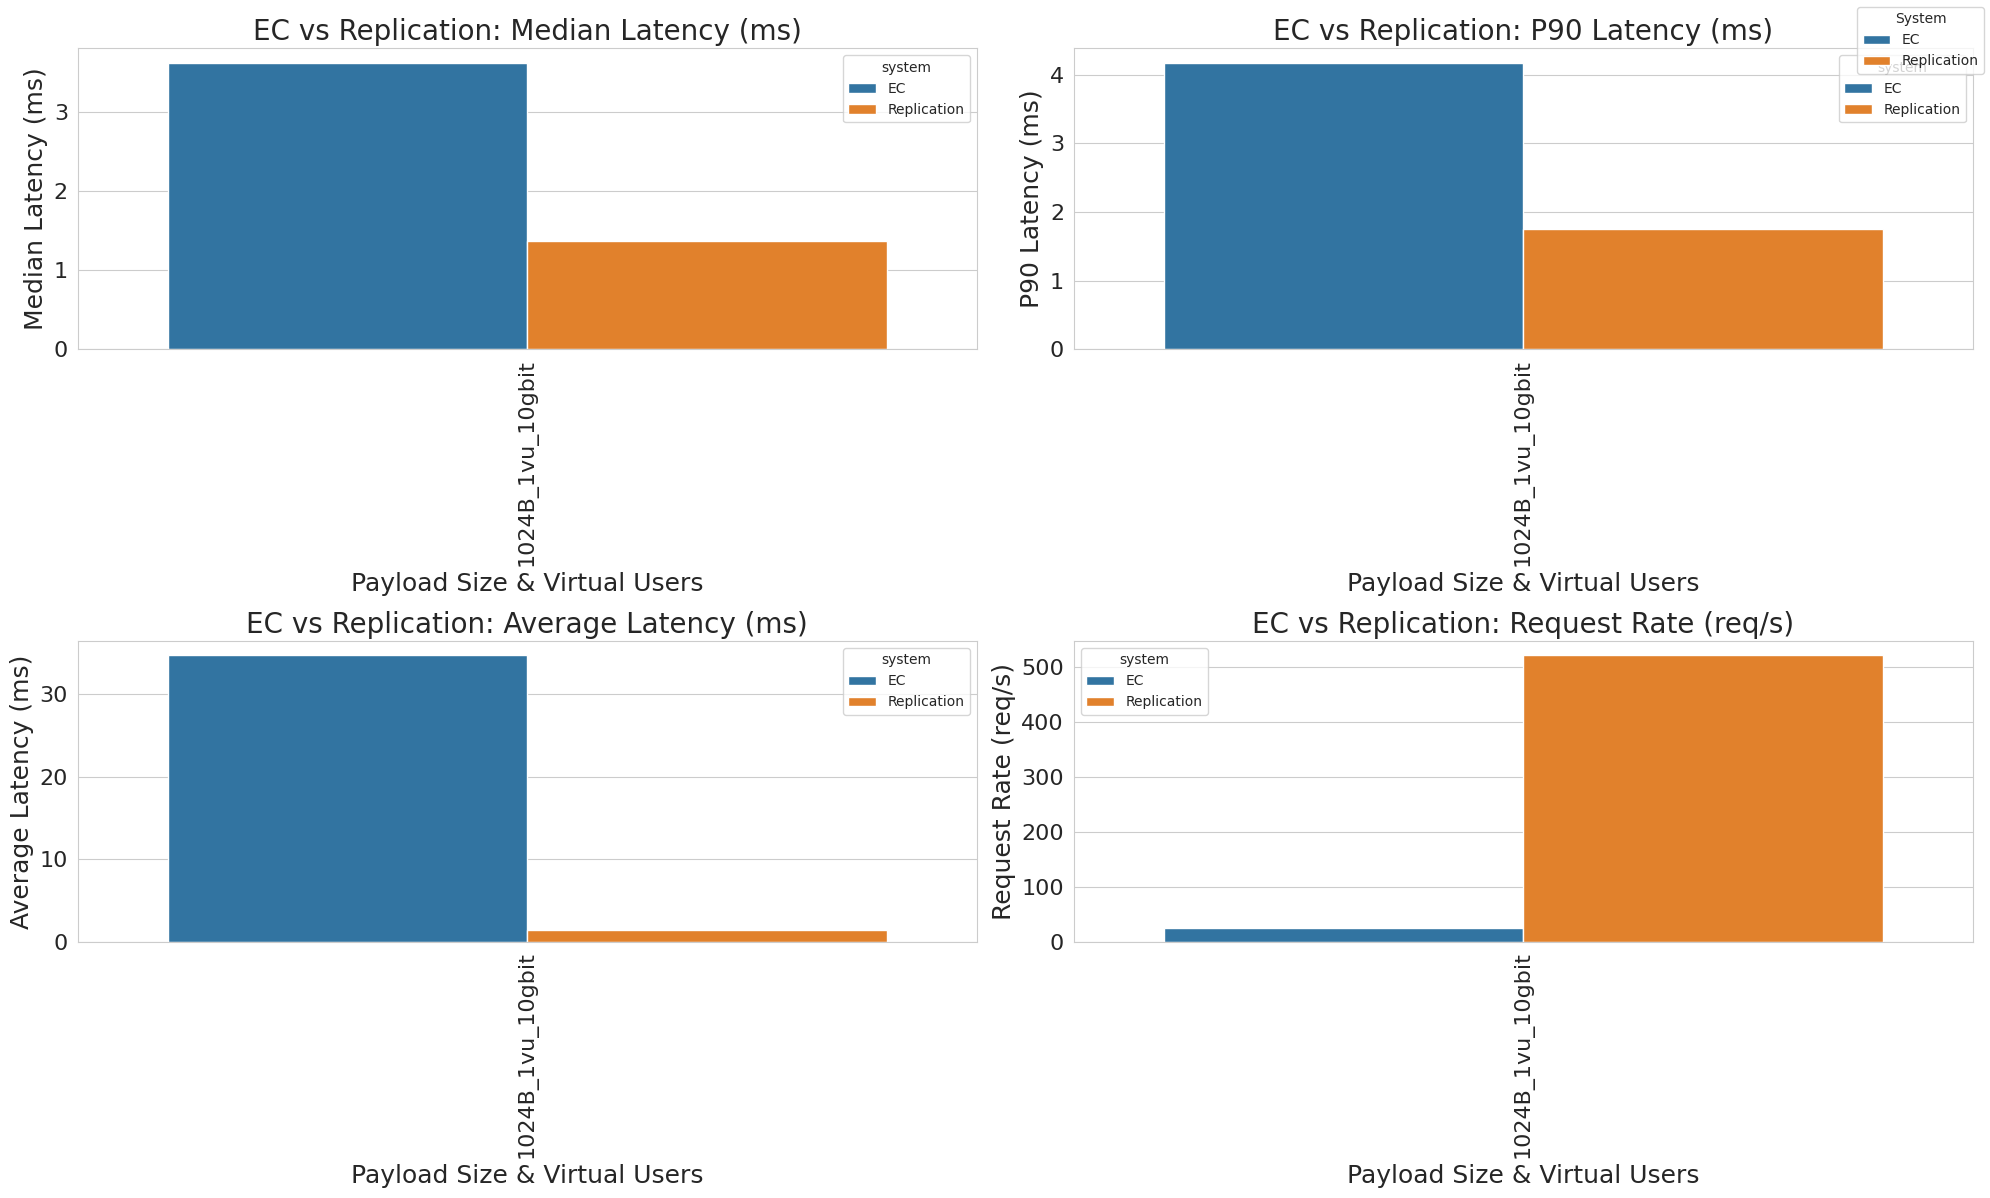
\includegraphics[width=0.8\textwidth]{resources/chapter-4/read_smload_fastnet.png}

    \caption{Kinerja Operasi Read pada Internet Cepat dan Payload Kecil}
      \label{fig:read-smload-fastnet}
  \end{figure}

  Proses \textit{erasure coding} memerlukan rekonstruksi data sehingga kinerjanya selalu lebih lambat dibandingkan replikasi. Grafik tersebut memperlihatkan kinerja \textit{erasure coding} dan replikasi memiliki perbedaan yang signifikan.

  \item Skenario 2: Internet lambat dan \textit{payload} besar
  
  Skenario kedua berlawanan dengan skenario pertama pada operasi \textit{write}. Namun, kondisi ini tidak berlaku untuk operasi \textit{read}. Gambar \ref{fig:read-bigload-slownet} menunjukkan hasil \textit{benchmark} untuk skenario ini.

  \begin{figure}[ht]
    \centering
    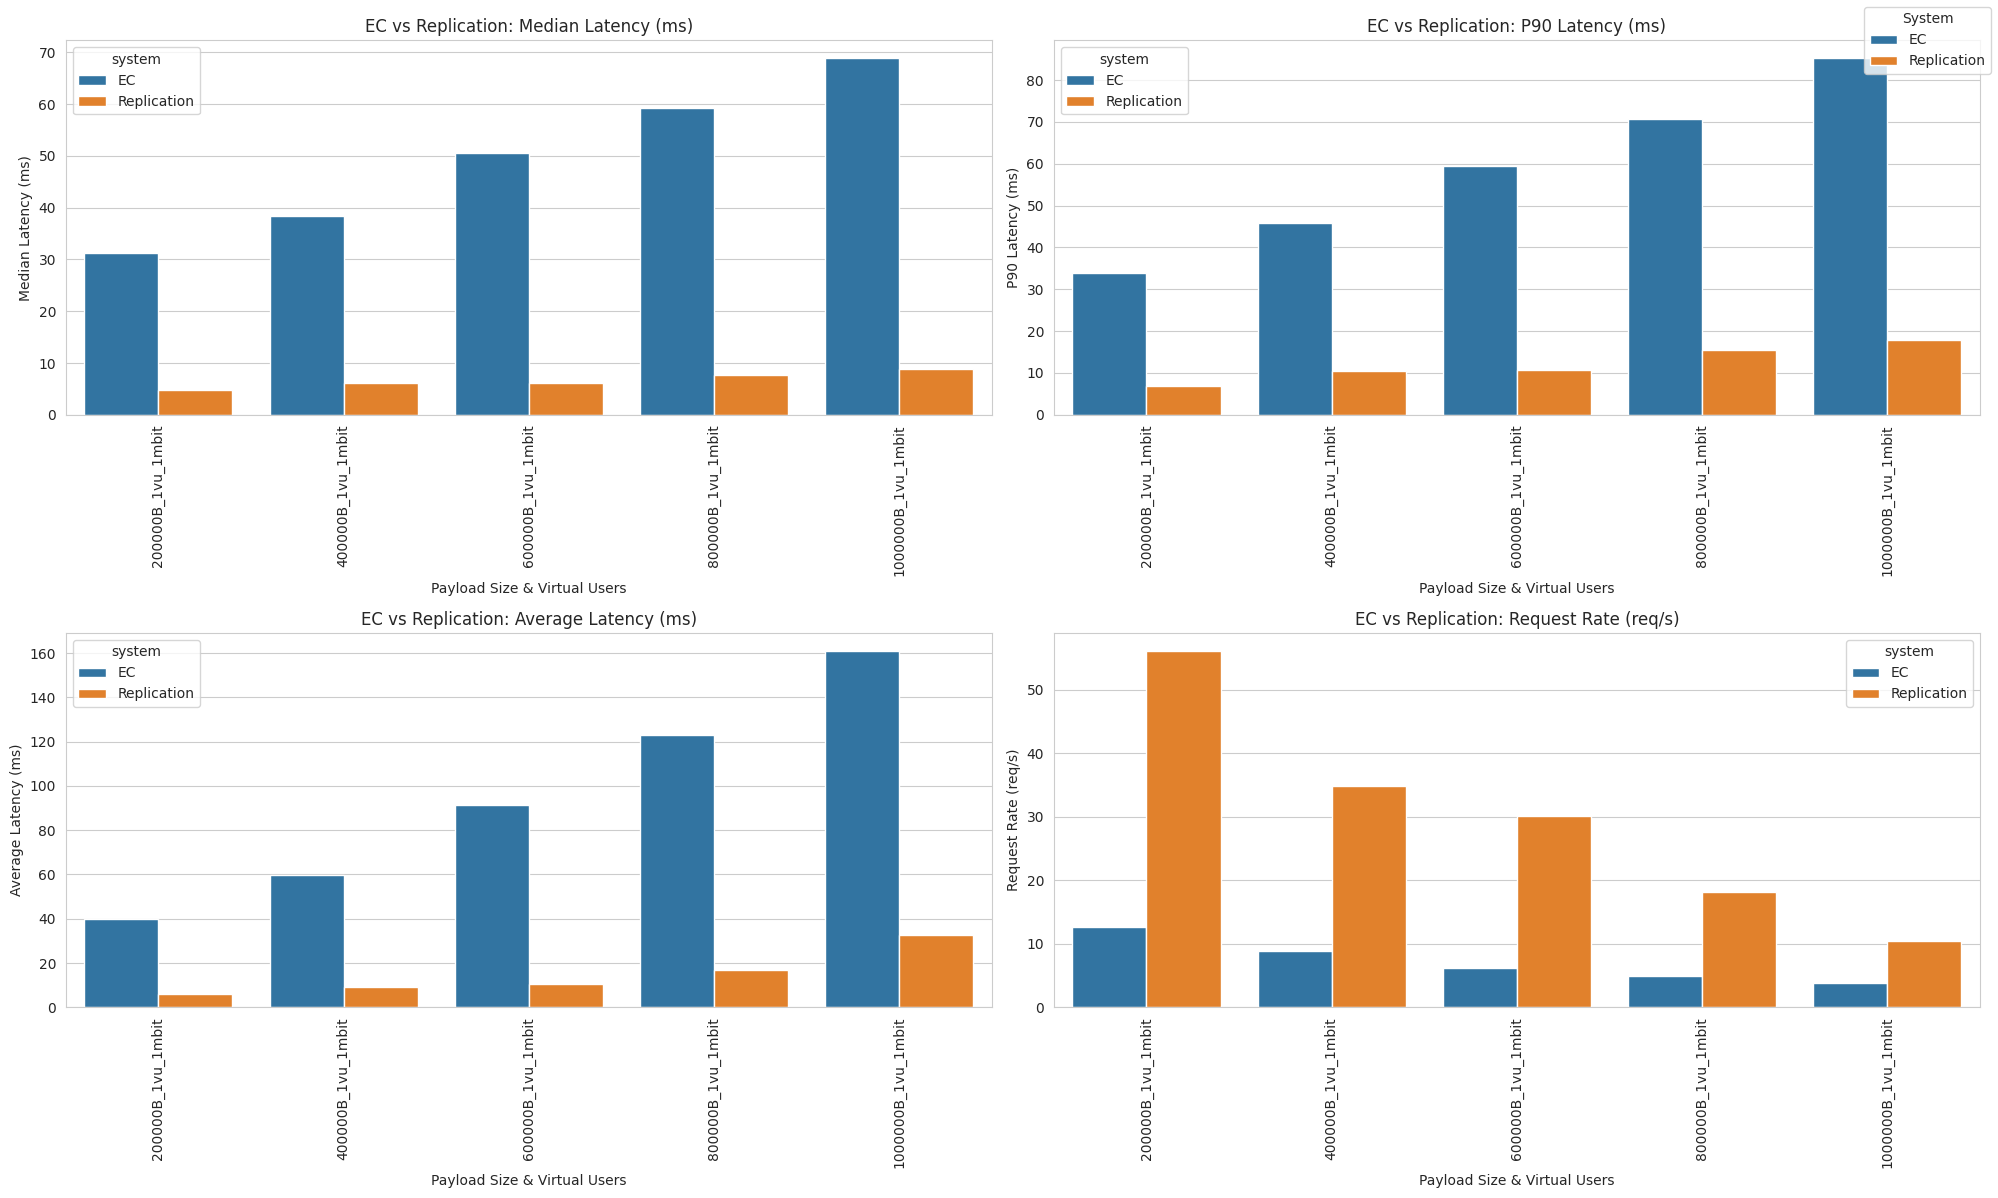
\includegraphics[width=0.8\textwidth]{resources/chapter-4/read_bigload_slownet.png}

    \caption{Kinerja Operasi Read pada Internet Lambat dan Payload Besar}
      \label{fig:read-bigload-slownet}
  \end{figure}

  Hasil dari skenario ini mengkonfirmasi bahwa \textit{erasure coding} tidak dapat mengungguli replikasi dalam kondisi apapun untuk operasi \textit{read}. Proses rekonstruksi data pada sistem \textit{erasure coding} akan tetap membutuhkan waktu yang lebih lama dibandingkan dengan replikasi, meskipun dalam kondisi internet lambat dan \textit{payload} besar. Selain itu, hasil ini menunjukkan juga bahwa keuntungan yang dimiliki \textit{erasure coding} dalam operasi \textit{write} perlu diiringi dengan penurunan kinerja pada operasi \textit{read}.

  \item Skenario 3: Internet menengah dan \textit{payload} besar
  
  Dari konfirmasi yang didapatkan dari kedua skenario sebelumnya bahwa \textit{erasure coding} tidak dapat mengungguli replilkasi untuk operasi \textit{read} dalam kondisi apapun, skenario ketiga melakukan eksplorasi tambahan terkait signifikansi perbedaan kinerja antar \textit{erasure coding} dan replikasi. Gambar \ref{fig:read-bigload-avgnet} menunjukkan hasil \textit{benchmark} untuk skenario ini.

  \begin{figure}[ht]
    \centering
    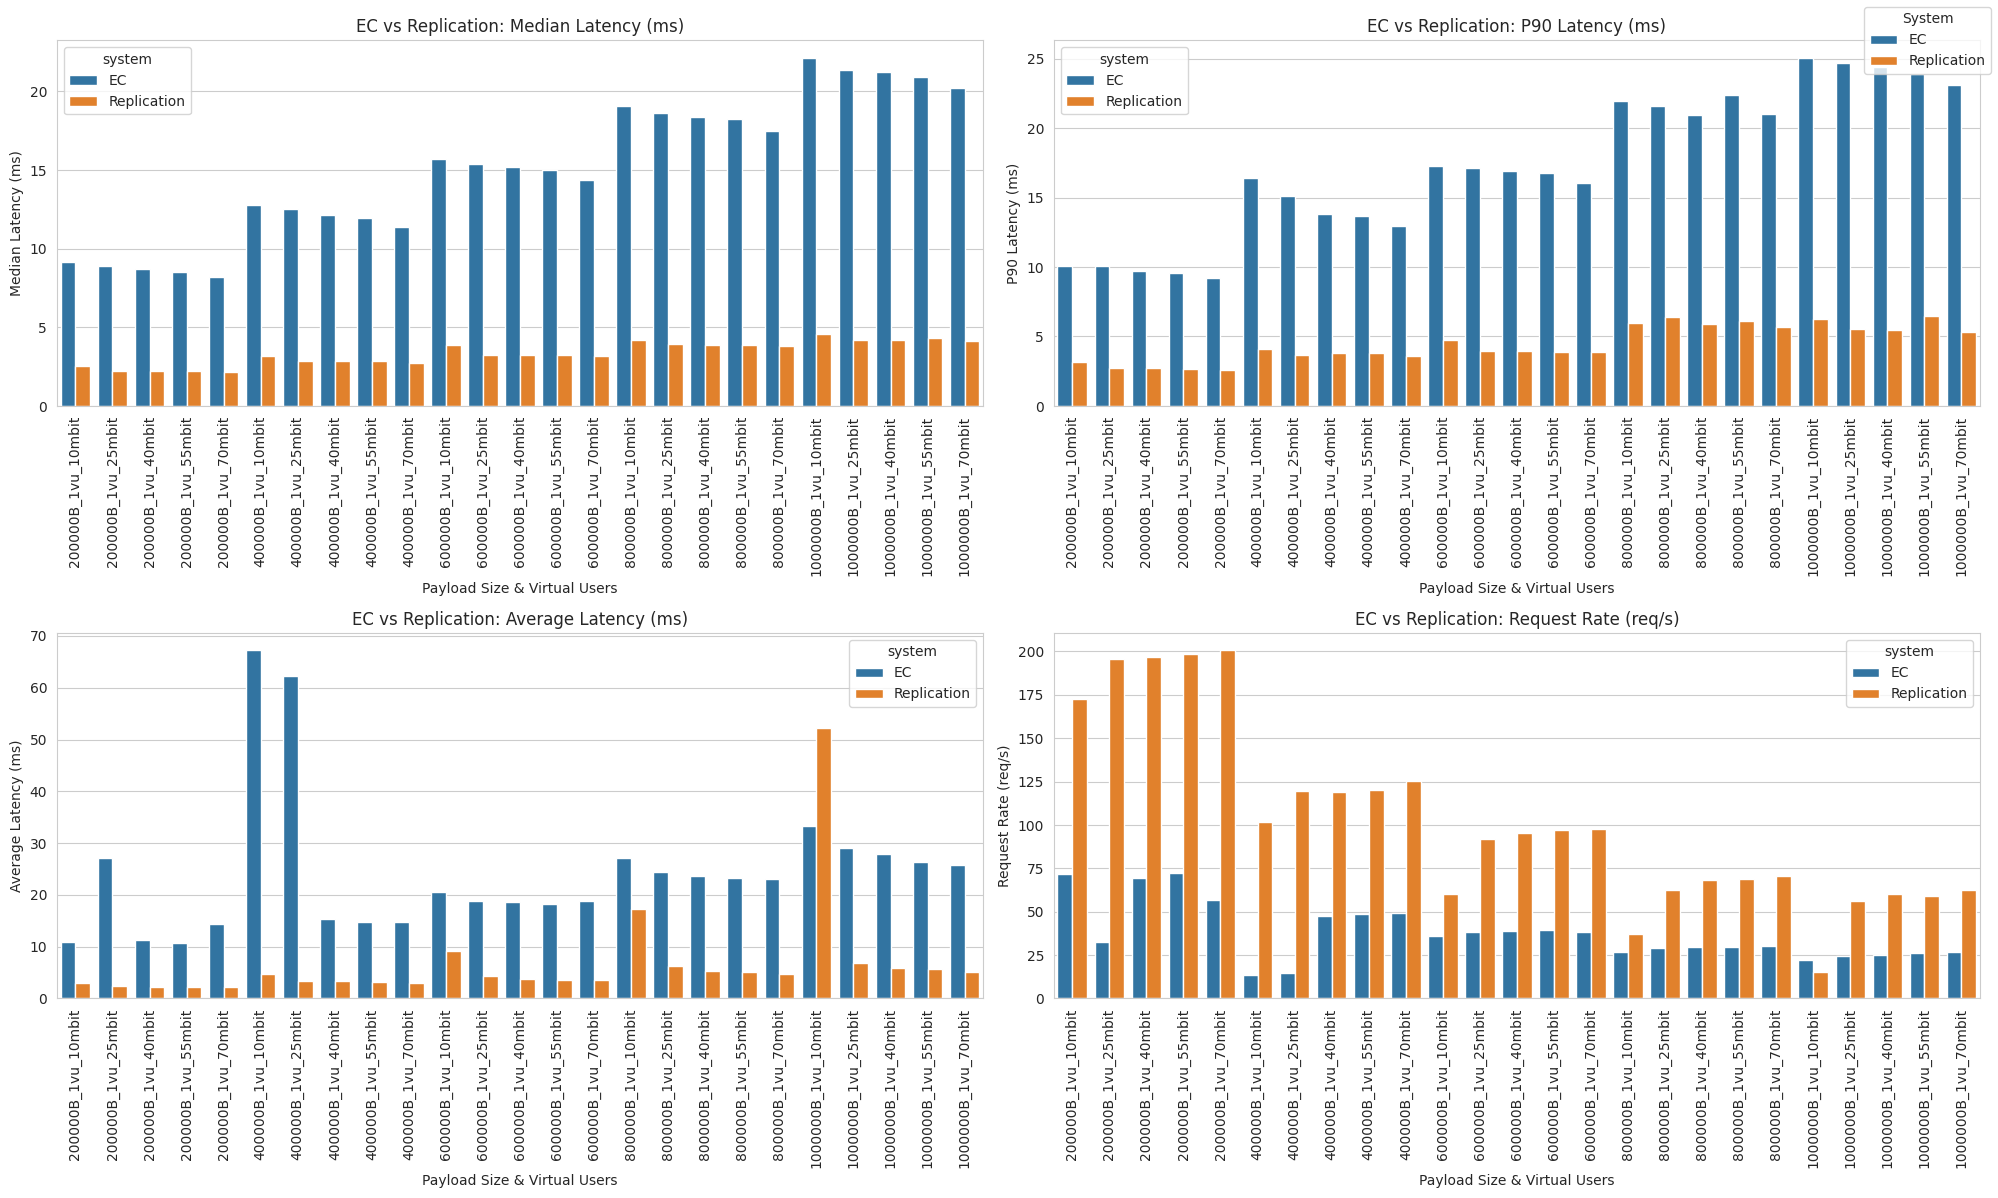
\includegraphics[width=0.8\textwidth]{resources/chapter-4/read_bigload_avgnet.png}

    \caption{Kinerja Operasi Read pada Internet Menengah dan Payload Besar}
      \label{fig:read-bigload-avgnet}
  \end{figure}

  Mengabaikan data \textit{noise} hasil \textit{benchmark}. Grafik tersebut menunjukkan perbedaan kinerja antara sistem berbasis \textit{erasure coding} dan replikasi secara umum menurun dengan \textit{payload} yang lebih kecil. Hal ini disebabkan oleh proses rekonstruksi data berjalan lebih cepat ketika \textit{payload} yang direkonstruksi lebih kecil dengan berkurangnya operasi yang perlu dilakukan dan juga pengiriman data antar-\textit{node}.

  Visualisasi \textit{heatmap} pada Gambar \ref{fig:read-bigload-avgnet-heatmap} menunjukkan perbedaan kinerja replikasi unggul pada operasi \textit{read}. Keunggulan ini semakin bertambah ketika \textit{payload} yang direkonstruksi semakin besar. Perubahan \textit{bandwidth} juga mempengaruhi kinerja \textit{erasure coding} dan replikasi. Penambahan \textit{bandwidth} menambah \textit{response time} dari kedua sistem, namun \textit{erasure coding} terlihat lebih terpengaruh dibandingkan replikasi. Hal ini disebabkan oleh proses rekonstruksi data yang membutuhkan pengumpulan \textit{fragment} dari beberapa \textit{node} terpisah terlebih dahulu melalui jaringan sebelum melakukan rekonstruksi, sedangkan replikasi hanya bertambah waktu yang diperlukan untuk mengirimkan data dari \textit{node} ke \textit{client}. Kode untuk visualisasi \textit{heatmap} dapat dilihat pada repository Github hasil implementasi.

  \begin{figure}[ht]
    \centering
    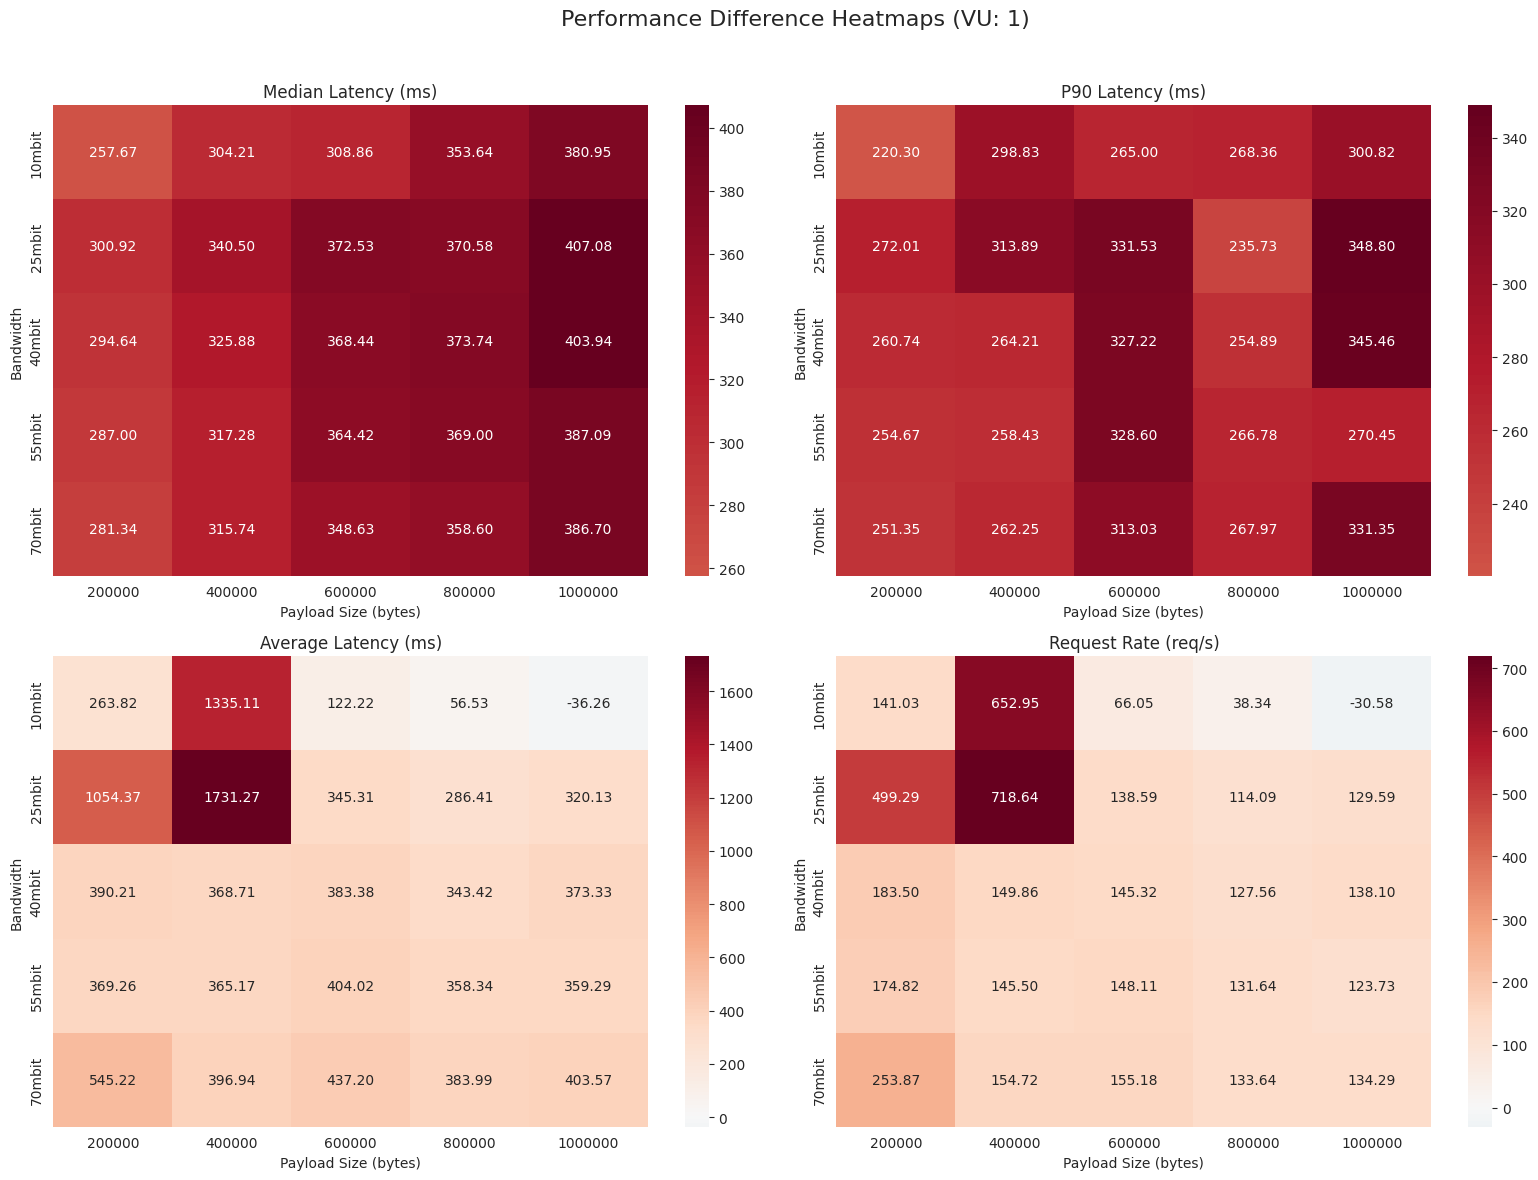
\includegraphics[width=0.8\textwidth]{resources/chapter-4/read_bigload_avgnet_heatmap.png}

    \caption{Heatmap Read pada Internet Menengah dan Payload Besar}
      \label{fig:read-bigload-avgnet-heatmap}
  \end{figure}

  Jike dibentuk diagram garis untuk memvisualisasikan pendekatan kinerja operasi \textit{read} pada sistem berbasis \textit{erasure coding} dan replikasi. Terlihat bahwa diagram garis yang dibentuk tidak menunjukkan \textit{trajectory} bahwa garis akan bersinggungan dengan garis \textit{erasure coding} pada titik tertentu. Perbandingan kinerja replikasi dan \textit{erasure coding} pada operasi \textit{read} memiliki kurva yang berbeda dan tidak akan bersinggungan. Diagram garis ini dapat dilihat pada Gambar \ref{fig:read-bigload-avgnet-line}.

  \begin{figure}[ht]
    \centering
    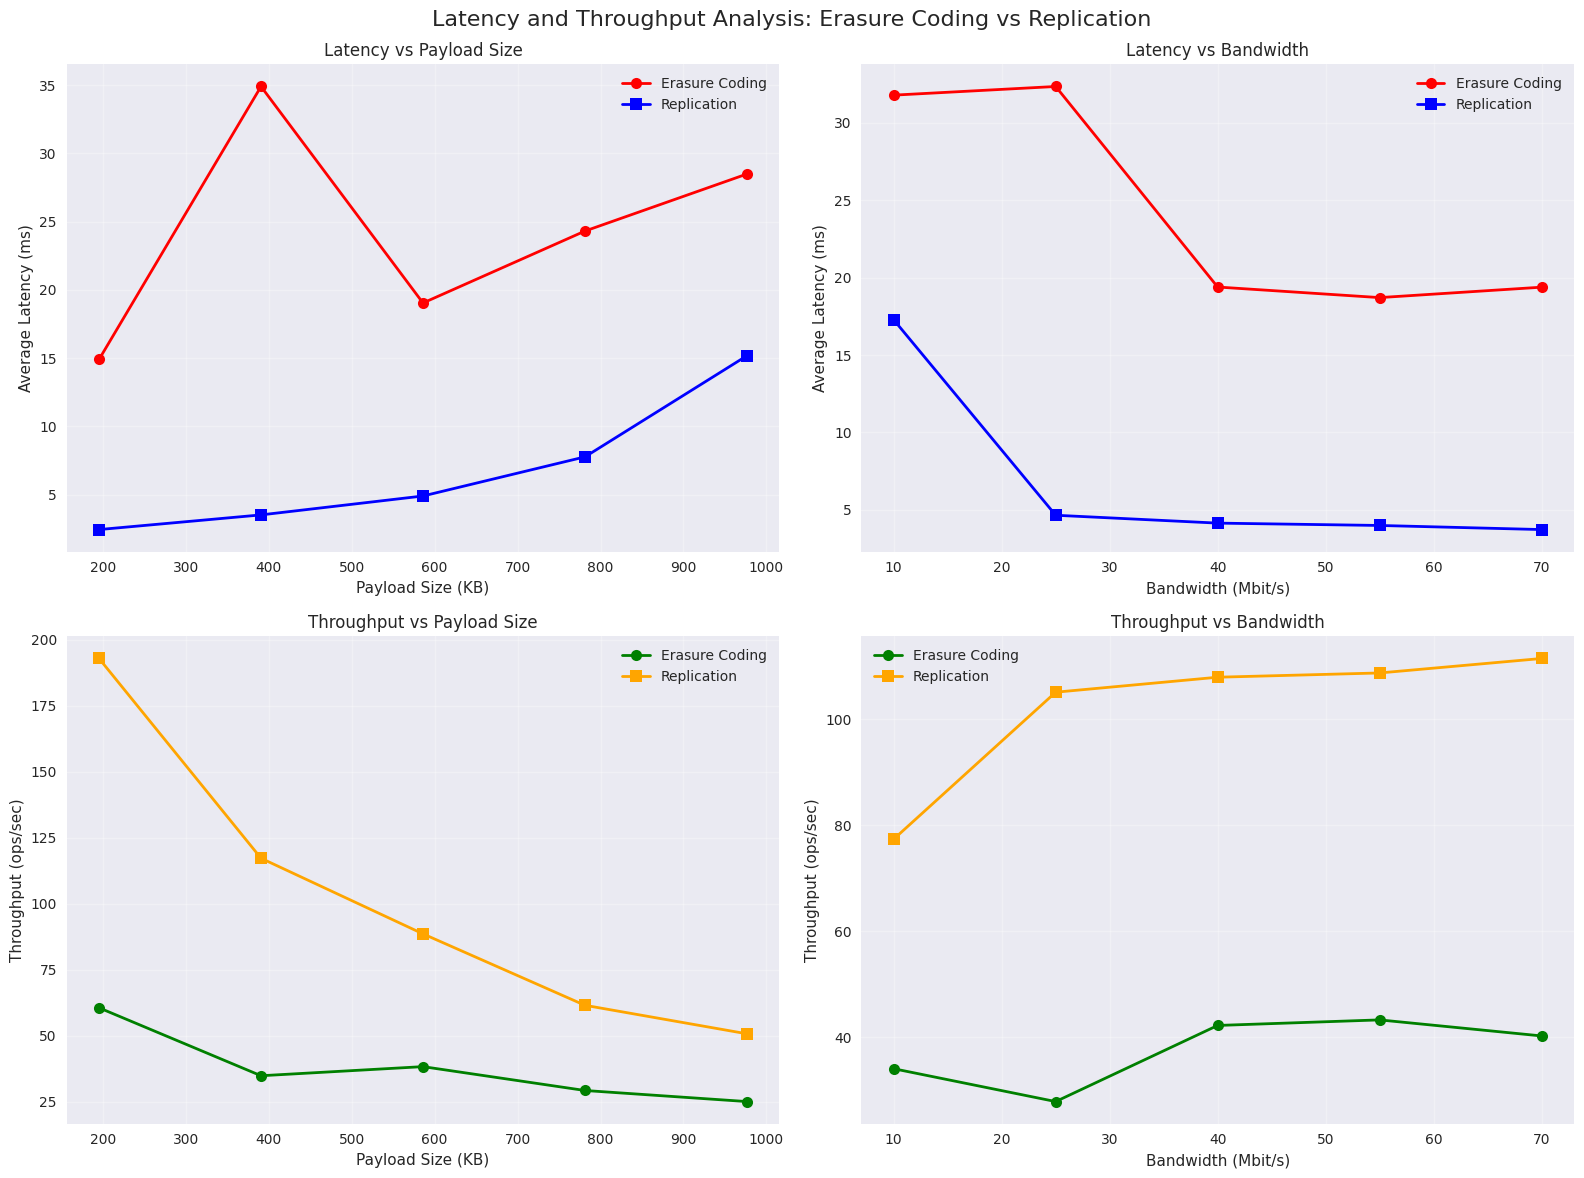
\includegraphics[width=0.8\textwidth]{resources/chapter-4/read_bigload_avgnet_line.png}

    \caption{Diagram Garis Read pada Internet Menengah dan Payload Besar}
    \label{fig:read-bigload-avgnet-line}
  \end{figure}

  Pembuktian matematis sederhana dapat dilakukan untuk menyatakan bahwa kinerja \textit{erasure coding} tidak akan pernah mengungguli replikasi pada operasi \textit{read}. Erasure coding akan membutuhkan waktu untuk memberikan data pada \textit{client}, rekonstruksi, dan meminta \textit{shard} pada \textit{node} lainnya, sedangkan replikasi hanya membutuhkan waktu untuk memberikan data pada \textit{client}. Persamaan \ref{eq:ec-read-latency} dan Persamaan \ref{eq:rep-read-latency} menunjukkan perhitungan latensi operasi \textit{read} pada sistem berbasis \textit{erasure coding}.

  \begin{align}
  L_{EC} &= T_{data} + T_{rekonstruksi} + T_{shard}
  \label{eq:ec-read-latency}
  \end{align}

  Sementara itu, Persamaan \ref{eq:rep-read-latency} menunjukkan perhitungan latensi operasi \textit{read} pada sistem berbasis replikasi.

  \begin{align}
  L_{REP} &= T_{data}
  \label{eq:rep-read-latency}
  \end{align}

  Dari persamaan tersebut, waktu antara \textit{erasure coding} dan replikasi dapat dituliskan sebagai Persamaan \ref{eq:read-latency-diff}.

  \begin{align}
  \Delta L &= L_{EC} - L_{REP} \\
  &= (T_{data} + T_{rekonstruksi} + T_{shard}) - T_{data} \\
  &= T_{rekonstruksi} + T_{shard}
  \label{eq:read-latency-diff}
  \end{align}

  Dengan demikian, perbedaan waktu antara \textit{erasure coding} dan replikasi akan menjadi semakin besar relatif terhadap ukuran data ketika data direkonstruksi, ukuran data ketika pengiriman data, dan juga \textit{bandwidth} yang tersedia ketika pengiriman data.
  
  Penambahan \textit{in-memory store} akan menghilangkan penambahan waktu ini. Namun, tidak semua \textit{request} dapat dilayani menggunakan \textit{in-memory store} karena keterbatasan memory yang tersedia. Oleh karena itu, peningkatan kinerja \textit{in-memory store} relatif terhadap rasio \textit{hit} dan \textit{miss} dari \textit{key} yang diminta. Jika \textit{hit} adalah seratus persen, maka \textit{erasure coding} akan memiliki kinerja yang setara dengan replikasi. Penambahan \textit{in-memory store} memodifikasi Persamaan \ref{eq:ec-read-latency} menjadi Persamaan \ref{eq:ec-read-latency-inmemory}.

  \begin{align}
    L_{EC} &= T_{data} + (T_{rekonstruksi} + T_{shard}) \times (1 - \text{hit rate})
    \label{eq:ec-read-latency-inmemory}
  \end{align}

  Dari persamaan tersebut, penambahan waktu yang dibutuhkan untuk operasi \textit{read} pada sistem berbasis \textit{erasure coding} dapat dihitung dengan mengurangi waktu yang dibutuhkan untuk operasi \textit{read} pada sistem replikasi. Persamaan ini dapat dituliskan sebagai Persamaan \ref{eq:ec-read-latency-diff-inmemory}.

  \begin{align}
    \Delta L &= L_{EC} - L_{REP} \\
    &= \left[T_{data} + (T_{rekonstruksi} + T_{shard}) \times (1 - \text{hit rate})\right] - T_{data} \\
    &= (T_{rekonstruksi} + T_{shard}) \times (1 - \text{hit rate})
    \label{eq:ec-read-latency-diff-inmemory}
  \end{align}

  Penambahan \textit{in-memory store} akan mengurangi waktu operasi \textit{read} pada sistem berbasis \textit{erasure coding} dengan kemungkinan untuk mengimbangi kinerja replikasi. Namun, hal ini tergantung pada rasio \textit{hit} yang dapat dicapai oleh \textit{in-memory store}.
  
  % Jika analisis regresi yang mirip dengan analisis pada Bagian \ref{subsubsection:analisis-operasi-write} dilakukan, hasil menunjukkan bahwa untuk semua skenario, \textit{erasure coding} memiliki kinerja yang lebih lambat dibandingkan replikasi. Grafik akhir dari analisis ini dapat dilihat pada Gambar \ref{fig:read-bigload-avgnet-regression}. Perlu diamati juga bahwa nilai \textit{R-squared} yang didapatkan dari analisis regresi ini adalah ada di bawah 0.5, yang menunjukkan bahwa model regresi ini tidak dapat menjelaskan variasi data dengan baik. Hal ini sebagian besar disebabkan oleh adanya \textit{noise} yang tinggi pada hasil \textit{benchmark}.

  % \begin{figure}[ht]
  %   \centering
  %   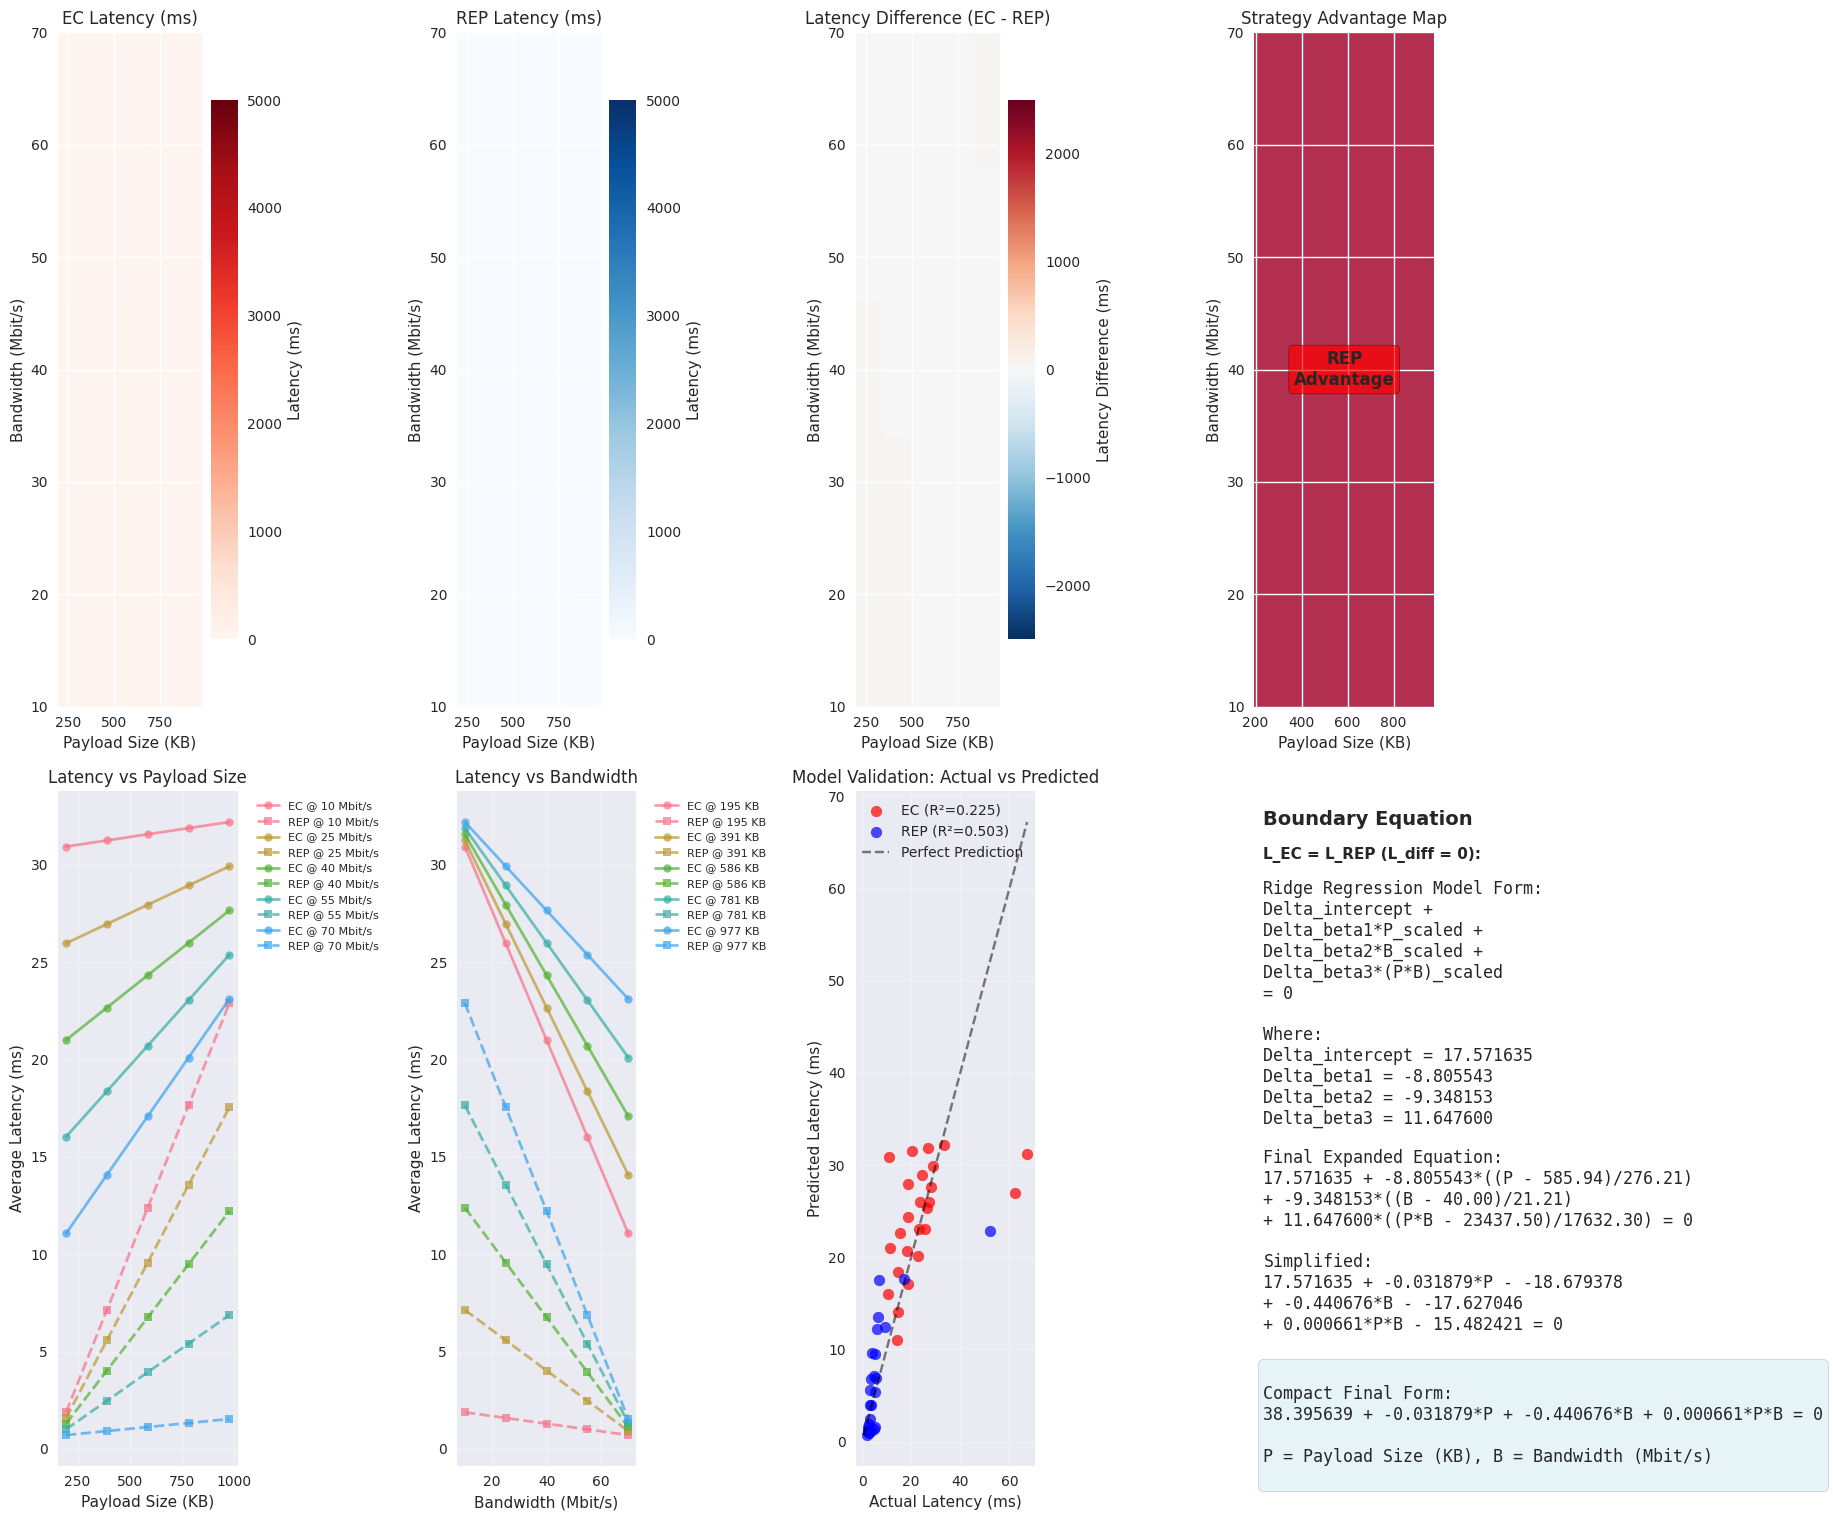
\includegraphics[width=0.8\textwidth]{resources/chapter-4/read_bigload_avgnet_regression.png}

  %   \caption{Analisis Regresi Read pada Internet Menengah dan Payload Besar}
  %   \label{fig:read-bigload-avgnet-regression}
  % \end{figure}
\end{enumerate}
\subsubsection{Analisis Keseluruhan}
\label{subsubsection:analisis-keseluruhan}

Setelah melakukan analisis terhadap dua operasi \textit{write} dan \textit{read}, bagian analisis ini menyatukan temuan dari evaluasi kinerja operasi tersebut. Tujuannya menyajikan gambaran keseluruhan mengenai \textit{trade-off} fundamental antara \textit{erasure coding} dan replikasi.

Hasil penelitian ini menunjukkan bahwa untuk kedua sistem:
\begin{enumerate}
  \item \textit{Erasure Coding}
  
  Sistem berbasis \textit{erasure coding} selain menawarkan efisiensi penyimpanan yang superior dibandingkan replikasi, juga memiliki keunggulan dalam hal latensi operasi \textit{write} pada beban kerja tertentu. Beban kerja yang dimaksud adalah ketika ukuran data cukup besar dan \textit{bandwidth} jaringan yang tersedia terbatas.

  \item Replikasi
  
  Sistem berbasis replikasi menawarkan kinerja operasi \textit{write} yang lebih baik pada beban kerja dengan ukuran data kecil dan \textit{bandwidth} jaringan yang tinggi. Selain itu, replikasi juga unggul dalam operasi \textit{read}. Perlu diperhatikan bahwa replikasi membutuhkan biaya penyimpanan yang lebih tinggi dibandingkan \textit{erasure coding}.

\end{enumerate}

Dalam penggunaannya \textit{erasure coding} dan replikasi memiliki kelebihan dan kekurangan masing-masing. Penggunaan \textit{erasure coding} lebih cocok untuk sistem yang memprioritaskan efisiensi penyimpanan dan toleransi kegagalan, sedangkan replikasi lebih sesuai untuk sistem yang mengutamakan kinerja operasi \textit{read} dan \textit{write} pada beban kerja dengan ukuran data kecil.

Pemilihan penggunaan kedua sistem perlu mempertimbangkan karakteristik beban kerja, rasio baca dan tulis, ukuran data, dan infrastruktur jaringan yang tersedia. Dalam \textit{key-value store} yang lazim beroperasi dengan data kecil dan menggunakan infrastruktur \textit{data center} ber-\textit{bandwidth} tinggi, replikasi akan menjadi pilihan yang lebih baik. Namun, untuk sistem yang menangani data besar dan memerlukan efisiensi penyimpanan, dan berinfrastruktur terbatas, \textit{erasure coding} akan lebih diuntungkan.
